\documentclass[11pt]{article}
\usepackage{CJKutf8}
\usepackage{indentfirst}
\usepackage{amsmath}
\usepackage{graphicx}
\usepackage{geometry}
\usepackage{fancyhdr}
\usepackage{comment}
\usepackage{listings}
\usepackage{algorithm}
\usepackage{color}
\usepackage{algorithmic}
\usepackage{setspace} % 行间距
\usepackage{float}
\usepackage{graphicx}
\graphicspath{{Problems/}}
\usepackage{verbatim}
\usepackage{tikz}
\usetikzlibrary{shadows}
\usepackage{verbatim}
\usepackage{pgfplots}
\usepackage{verbatim}
\usetikzlibrary{arrows,shapes}
\usepackage{epstopdf}

\definecolor{darkblue}{rgb}{0.2,0.2,0.6}
\definecolor{darkred}{rgb}{0.6,0.1,0.1}
\definecolor{darkgreen}{rgb}{0.2,0.6,0.2}

\usetikzlibrary{shadings,shadows,shapes.arrows}

\usetikzlibrary{calc}

\tikzstyle{vertex}=[circle,fill=black!25,draw,minimum size=20pt,inner sep=0pt]
\tikzstyle{middlevertex}=[circle,fill=black!25,draw,minimum size=15pt,inner sep=0pt]
\tikzstyle{smallvertex}=[circle,fill=black!25,draw,minimum size=10pt,inner sep=0pt]
\tikzstyle{selected vertex} = [vertex, draw,fill=red!24]
\tikzstyle{blue smallvertex} = [smallvertex, draw,fill=blue]
\tikzstyle{red smallvertex} = [smallvertex, draw,fill=red]
\tikzstyle{edge} = [draw,thick,->]
\tikzstyle{undirectededge} = [draw,thick]
\tikzstyle{weight} = [font=\small]
\tikzstyle{selected edge} = [draw,line width=5pt,-,red!50]
\tikzstyle{ignored edge} = [draw,line width=5pt,-,black!20]


\title{\textbf{算法第9讲}}
\author{孔鲁鹏}
\date{2015-12-6}
%设置页边距
\geometry{papersize={21cm,29.7cm}}  %长,宽
\geometry{left=2.54cm,right=2.54cm,top=2.54cm,bottom=2.54cm} %左右上下边距

\onehalfspacing  %将行距设置为 1.5 倍:

%设置页眉页脚
\pagestyle{fancy}
\lhead{}       %左页眉
\chead{}
\rhead{}
\lfoot{}	 %左页脚
\cfoot{}
\rfoot{}
\renewcommand{\headrulewidth}{0.4pt}
\renewcommand{\headwidth}{\textwidth}
\renewcommand{\footrulewidth}{0pt}
%首行缩进
\setlength{\parindent}{2em}

\begin{document}
\begin{CJK}{UTF8}{gbsn}
\maketitle
\section{原始对偶算法}
\subsection{原始对偶算法引入}
今天我们讲一个很重要的technique,叫原始对偶。原始对偶也是一种迭代式的,逐步改进式的迭代方法。这两节课都比较难,但是当你觉得它有用的时候,你就会觉得它不这么难了。原始对偶方法也是一种对偶方法,他也要解一个对偶。它充分利用问题的下界信息。原始对偶和原来的对偶单纯型不太一样,它不像对偶单纯型,一定要从一个对偶基可行解出发。原始对偶方法只要求对偶可行就行。第二,在原始对偶方法中,每次都要迭代解一个DRP。DRP是一个小线性规划,但很多时候,我们不用单纯型去解它。因为它有很多的直观的组合解释,尤其对于图论问题。
\subsection{原始对偶算法}


\textbf{原始对偶算法基本思路:}

我们用这幅图来说明原始对偶方法:

\begin{figure}[H]
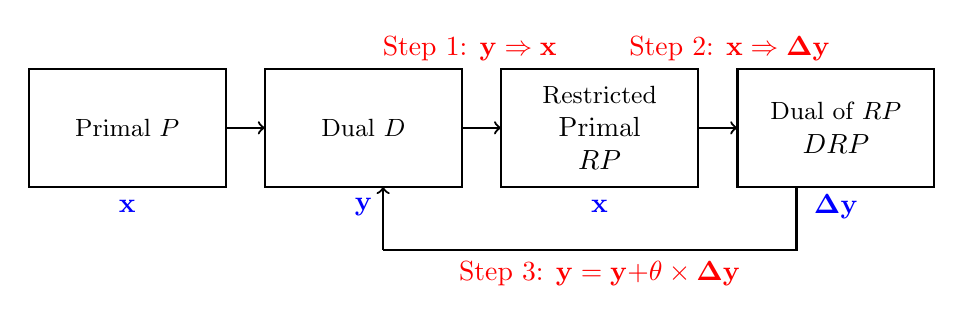
\begin{tikzpicture}[scale=1., auto,swap]

\def\l{2.5};
\def\h{1.5};
\def\d{0.5};

\draw[thick] (0,0) rectangle (\l,\h);
\draw[thick, ->] (\l, \h*0.5) -- ( \l + \d, \h*0.5);
\node[ultra thick] at (\l*0.5, \h*0.5) {\small Primal $P$};
\node[thick, blue] at (\l*0.5 , -0.25) {$\mathbf{x}$};

\node[thick, red] at (\l + \d + \l + \d*0.2 , \h + 0.25 ) {Step $1$: $\mathbf{y\Rightarrow x}$};


\draw[thick] (0 + \l + \d, 0) rectangle (\l + \l + \d,\h);
\draw[thick, ->] (\l + \l + \d , \h*0.5) -- ( \l + \d + \l + \d, \h*0.5);
\node[ultra thick] at (\l+\d + \l*0.5, \h*0.5) {\small Dual  $D$};
\node[thick, blue] at (\l+\d + \l*0.5, -0.25) {$\mathbf{y}$};

\node[thick, red] at (\l + \d + \l + \d + \l + \d*0.8 , \h + 0.25 ) {Step $2$: $\mathbf{x}\Rightarrow \mathbf{\Delta y}$};


\draw[thick] (0 + \l + \d + \l + \d, 0) rectangle (\l + \l + \d+ \l + \d,\h);
\draw[thick, ->] (\l + \l + \d + \l + \d, \h*0.5) -- ( \l + \d + \l + \d + \l + \d, \h*0.5);
\node[ultra thick, align=center] at (\l+\d + \l+\d + \l*0.5,  \h*0.5) {\small Restricted\\ Primal\\ $RP$};
\node[thick, blue] at (\l+\d + \l+\d + \l*0.5,  -0.25) {$\mathbf{x}$};

\node[thick, red] at (\l+\d + \l+\d + \l*0.5,  -1.1) { Step $3$: $\mathbf{y = y + }\theta \times \mathbf{\Delta y}$};


\draw[thick] (0 + \l + \d + \l + \d + \l + \d, 0) rectangle (\l + \l + \d+ \l + \d + \l + \d,\h);
\node[ultra thick, align=center] at (\l+\d + \l+\d + \l+\d + \l*0.5 , \h*0.5) {\small Dual of $RP$\\ $DRP$};
\node[thick, blue] at (\l+\d + \l+\d + \l+\d + \l*0.5 , -0.25) {$\mathbf{\Delta y}$};

\draw[thick] (\l+\d + \l+\d + \l+\d + \l*0.3 , 0) -- (\l+\d + \l+\d + \l+\d + \l*0.3 , -0.8) -- (\l+\d + \l*0.6, -0.8);
\draw[thick, ->]  (\l+\d + \l*0.6, -0.8) --  (\l+\d + \l*0.6, 0);


\end{tikzpicture}
\end{figure}

假如我们要求解远线性规划问题P,它的变量是X。我们先把它的对偶问题写出来。假如我们拿到对偶问题的一个可行解Y,我们把Y带入到对偶问题中,看看Y能指导我们得到X多少的信息,得到的X的信息又能够知道我们如何改进Y。通过这样不断迭代改进Y,找到最优解。这里有很多名词,大家先不要着急,一个个的看下去。


\textbf{得到RP}

看个例子。
\begin{itemize}
\begin{footnotesize}
\item
Primal P:
\[
\begin{array}{rrrrrrrrrrrrl}
 \min & c_1x_1    &+&  c_2x_2   &+&  ...&+& c_nx_n    &      &    & \\
 s.t. & a_{11}x_1 &+& a_{12}x_2 &+& ... &+& a_{1n}x_n & = & b_1 & \textcolor{blue}{(y_1)} \\
      & a_{21}x_1 &+& a_{22}x_2 &+& ... &+& a_{2n}x_n & = & b_2 & \textcolor{blue}{(y_2)} \\
      &           & &           & & ... & &           &      &     &  \\
      & a_{m1}x_1 &+& a_{m2}x_2 &+& ... &+& a_{mn}x_n & = & b_m &  \textcolor{blue}{(y_m)}\\
      &       x_1 &,&       x_2 &,& ... &,&       x_n & \geq & 0   &  \\
     \end{array} \nonumber
\]
\item
Dual D:
\[
\begin{array}{rrrrrrrrrrrrl}
 \max & b_1y_1    &+&  b_2y_2   &+&  ...&+& b_my_m    &      &    & \\
 s.t. & a_{11}y_1 &+& a_{21}y_2 &+& ... &+& a_{m1}y_m & \leq & c_1 &  \\
      & a_{12}y_1 &+& a_{22}y_2 &+& ... &+& a_{m2}y_m & \leq & c_2 &  \\
      &           & &           & & ... & &           &      &     &  \\
      & a_{1n}y_1 &+& a_{2n}y_2 &+& ... &+& a_{mn}y_m & \leq & c_n &
%      &       y_1 &,&       y_2 &,&     &,&       y_m & \leq\geq & 0   & \\
     \end{array} \nonumber
\]
\end{footnotesize}
\end{itemize}
原始问题如上所示,我们将它的对偶问题写出来。怎么写对偶呢,我们再重复一遍。对偶就是拉格朗日乘子,每一行的约束做一个拉格朗日乘子,就是变量,叫做y1,y2,……。然后写出对偶问题。

假如我们拿到了对偶问题的一个可行解y,我们首先验证y是不是最优解。如何验证呢?

首先,如果y是最优解,则x要满足一个条件。什么条件呢?就是这样一个条件:
\begin{itemize}
\begin{small}

\item Dual problem D:
\[
\begin{array}{rrrrrrrrrrrrl}
\max & b_1y_1    &+&  b_2y_2   &+&  ...&+& b_my_m    &      &    & \\
 s.t. & a_{11}y_1 &+& a_{21}y_2 &+& ... &+& a_{m1}y_m & \leq & c_1 &  \textcolor{blue}{('='\Rightarrow x_1 \geq 0 )} \\
      %& a_{12}y_1 &+& a_{22}y_2 &+& ... &+& a_{m2}y_m & \leq & c_2 &  ('='\Rightarrow x_2 \geq 0 )\\
      &           & &           & & ... & &           &      &     &  \\
      & a_{1n}y_1 &+& a_{2n}y_2 &+& ... &+& a_{mn}y_m & \leq & c_n &  \textcolor{blue}{ ('<'\Rightarrow x_n = 0 )}
%      &       y_1 &,&       y_2 &,&     &,&       y_m & \leq\geq & 0   & \\
     \end{array} \nonumber
\]
\end{small}
\end{itemize}
假如我们拿到一个y,我们把y带入对偶问题的约束中,对于每一条约束,如果约束1取等号,则相当于没有告诉我x1的任何信息,x1大于等于0是本来就已知的。如果约束n取小于号,大家回忆一下我们讲的互补松弛性,如果约束取小于,xn必定等于0。
我们用$J$表示满足等于号的约束:
 \begin{figure}[H]
 \includegraphics[width=2.5in] {L9-RP.png}
\end{figure}
我们回到原始问题,如果Y是一个最优解,那么红框内表示满足的等号约束,篮框内的取小于号,对应的xn=0。也就是说给我一个Y,如果是最优的,带进去,X必须要满足这些条件:
\begin{itemize}
\begin{small}
\item RP:
\[
\begin{array}{rrrrrrrrrrrrl}
 %\min & 0& \\
      & a_{11}x_1 &+& a_{12}x_2 &+& ... &+& a_{1n}x_n & = & b_1 &  \\
      & a_{21}x_1 &+& a_{22}x_2 &+& ... &+& a_{2n}x_n & = & b_2 & \\
      &           & &           & & ... & &           &      &     &  \\
      & a_{m1}x_1 &+& a_{m2}x_2 &+& ... &+& a_{mn}x_n & = & b_m & \\
      &           & &           & &     & &       \textcolor{blue}{x_i} & \textcolor{blue}{=} & 0   &\textcolor{blue}{ i\notin J} \\
      &           & &           & &     & &       \textcolor{red}{x_i} & \textcolor{red}{\geq} & 0   & \textcolor{red}{i\in J}
     \end{array} \nonumber
\]
\end{small}
\end{itemize}
我们只需要解这个限制性的原问题restricted primal (RP)就可以了。没有目标函数,只需要X满足这些约束就够了。
解这个不等式约束问题,我们把它转化成线性规划问题来做。加一些松弛变量:s1,s2,...,sm,变成下面这样一个问题:
\[
\begin{array}{rrrrrrrllllllllll}
 \min &\epsilon=&s_1    &+s_2   &...&+s_{m} &                   &    &                     &        & \\
 s.t.   &               &s_1    &           &   &            &+a_{11}x_1 &... &+a_{1n}x_{n} & =b_1 & \\
         &               &         &  s_2    &   &            &+a_{21}x_1 &... &+a_{2n}x_{n} & =b_2 & \\
         &               &         &           &...&            &                    &... &                     &          &\\
         &               &         &           &   & s_m    &+a_{m1}x_1 &... &+a_{mn}x_{n} & =b_m & \\
         &               &         &           &    &            &                         &   &\textcolor{blue}{x_i} & \textcolor{blue}{=  0}   &\textcolor{blue}{ i\notin J} \\
         &               &         &           &    &            &                         &    &\textcolor{red}{x_i}  &       \textcolor{red}{\geq  0}   & \textcolor{red}{i\in J} \\
         &               &         &           &     &            &                        &    &             s_i     & \geq 0 &  \forall i  \\
     \end{array} \nonumber
\]
最优值如果等于0,表明我们能找到一个X满足RP。如果最优值大于0,RP没有可行解,所以Y就不是最优解。


\textbf{如何求解RP:DRP}

现在,我们回顾一下。如果Y是最优解,对应的X满足原先的约束,并且有些Xi=0(蓝框内)。我们只要找到这些X,Y就是最优的。如何找这些X呢?求解RP对应的线性规划,当然,我们不一定需要直接去解RP对应的线性规划,我们解RP对应的线性规划的对偶($DRP$),也是等价的:
\begin{itemize}
\item $DRP$:
\[
\begin{array}{rrrrrrrrrrrrrrrrrrrrl}
\max & w &=& b_1y_1    &+&  b_2y_2   &+&  ...&+& b_my_m    &      &    & \\
 s.t. & & & a_{11}y_1 &+& a_{21}y_2 &+& ... &+& a_{m1}y_m & \leq & 0 &  \\
      & & & a_{12}y_1 &+& a_{22}y_2 &+& ... &+& a_{m2}y_m & \leq & 0 &  \\
      & & &          & &           & & ... & &           &      &     &  \\
      & & & a_{1|J|}y_1 &+& a_{2|J|}y_2 &+& ... &+& a_{m|J|}y_m & \leq & 0 & \\
      & & &      y_1 &,&       y_2 &,&     &,&       y_m & \leq & 1   & \\
     \end{array} \nonumber
\]
\end{itemize}
当最优值是0的时候,Y就是最优的。否则Y不是最优的。当Y不是最优时,应该怎么办。这个时候虽然Y不是最优,但是我们对这个问题的求解所花的功夫没有白费。它提供了有用的信息,它可以告诉我们怎么改进Y。


\textbf{DRP优化y}

为什么说我们求得的DRP的解可以改进Y的呢?
我们构造一个解:$\mathbf{y' = y +} \theta \mathbf{ \Delta y}, \theta > 0 $.
如果说它要是改进的话,我们只要理解两点。第一点目标函数的确是变大啦。第二点,y是满足约束的,y'也应该是满足约束的。

我们先看第一点。DRP问题的目标函数和对偶问题的目标函数是一样的。所以,如果DRP问题的目标函数能找到一个最优解,它是等于0的,那我们就已经stop了,如果是大于0的话,我们可以知道,$\mathbf{\Delta y^T b } = w_{OPT}  > 0$,  $\mathbf{y'^T b = y^T b } + \theta w_{OPT}  > \mathbf{ y^T b}$.

第二点,y本来是满足约束的,会不会变大以后就不满足约束了呢。
对于任意的$ j \in J$,  $a_{1j} \Delta y_1 + a_{2j}\Delta y_2 + ... + a_{mj}\Delta y_m  \leq  0$(依据DRP的约束). 所以我们有 $\mathbf{y'^Ta_j} = \mathbf{y^Ta_j} + \theta \mathbf{\Delta y^Ta_j} \leq \mathbf{c_j}$ 对于任意的 $\theta > 0$.
对于$j \notin J$,又分两种情况:

第一种,对于$\forall j \notin J, a_{1j} \Delta y_1 + a_{2j}\Delta y_2 + ... + a_{mj}\Delta y_m  \leq  0$:

$\mathbf{y'}$肯定是一个可行解,对于 $\forall \theta > 0$ ,$\forall 1 \leq j \leq n$:
 \begin{eqnarray}
&&  a_{1j}y'_1 + a_{2j}y'_2 + ... + a_{mj}y'_m \\
&=&a_{1j}y_1 + a_{2j}y_2 + ... + a_{mj}y_m \\
&+&\theta(a_{1j}\Delta{y_1} + a_{2j}\Delta{y_2} + ... + a_{mj}\Delta{y_m}) \\
&\leq& c_j
\end{eqnarray}
换句话说,对偶问题是无界的,原问题是不可行的。因为原问题的解可以任意大。

第二种,$\exists j \notin J, a_{1j} \Delta y_1 + a_{2j}\Delta y_2 + ... + a_{mj}\Delta y_m  >  0$:

我们可以设置$\theta \leq \frac{c_j - (a_{1j}y_1 + a_{2j}y_2 + ... + a_{mj}y_m) } {a_{1j}\Delta {y_1} + a_{2j}\Delta {y_2} + ... + a_{mj}\Delta {y_m}} = \frac{ \mathbf{c_j - y^Ta_j} }{ \mathbf{\Delta y^T a_j}  }$ 从而使得$\mathbf{y'^Ta_j} =\mathbf{y^Ta_j} + \theta \mathbf{\Delta y^Ta_j} \leq \mathbf{c_j}$.


\textbf{原始对偶算法}

讲完这些,原始对偶算法就出来啦:
\begin{itemize}
\item 原始对偶算法:
\begin{small}
\begin{algorithmic} [1]
\STATE Infeasible = ``No''\\
       Optimal = ``No''\\
        $\mathbf{y=y_{0}}$; \qquad //$\mathbf{y_{0}}$ is a feasible solution to the dual problem $D$
\WHILE{TRUE}
\STATE Finding tight constraints index $J$, and set corresponding $x_j = 0 $ for $ j\notin J$.
\STATE Thus we have a smaller RP.
\STATE Solve DRP. Denote the solution as $\Delta \mathbf{y}$.
\IF{DRP objective function $w_{OPT} =0$}
\STATE Optimal=``Yes''\\
\RETURN $y$;
\ENDIF
\IF{ $\mathbf{\Delta y^T a_j \leq 0} $ (for all $j \notin J$)}
\STATE Infeasible = ``Yes'';
\RETURN;
\ENDIF
\STATE Set $\theta = \min{ \frac{ \mathbf{c_j - y^Ta_j} }{ \mathbf{\Delta y^T a_j}}}$ for $\mathbf{\Delta y^T a_j}>0$, $j\notin J$.
\STATE Update $\mathbf{ y}$ as  $ \mathbf{ y = y + \theta \Delta y}$;
\ENDWHILE
\end{algorithmic}
\end{small}
\end{itemize}
下面我们看一下原始对偶算法的优点。

1. 原始对偶算法肯定会结束。如果用一些防止退化的规则的话,肯定会结束的。(如何使用Bland法则防止退化的slides放到了网上)

2. 我们会看到无论是RP还是DRP都不显式的依赖于c。实际上那个c已经表达在那个J当中了。J就是我们得到的那些约束。

这就导致了原始对偶算法的一个很重要的优点。那就是:RP经常是一个纯粹性的组合问题。在最短路径问题当中,RP可以直接转化为一个组合问题--连通可达性问题。
我们把一个可行解带到对偶问题后,约束域的约束分成了两部分。一部分约束取等于号(我们看到的图中的红框);另一部分取严格小于号(图中的蓝框),这一部分对应的Xi=0,这意味着这些约束将不需要再考虑。问题的规模一下子大大缩小。我们只需要考虑红框的问题。原始对偶的优势就在于,每次都把问题缩小一块儿。
我们现在比较一下对偶问题和DRP问题:
\begin{itemize}
\item 对偶问题:
\[
\begin{array}{rrrrrrrrrrrrl}
\max & b_1y_1    &+&  b_2y_2   &+&  ...&+& b_my_m    &      &    & \\
 s.t. & a_{11}y_1 &+& a_{21}y_2 &+& ... &+& a_{m1}y_m & \leq & c_1 &   \\
      & a_{12}y_1 &+& a_{22}y_2 &+& ... &+& a_{m2}y_m & \leq & c_2 & \\
      &           & &           & & ... & &           &      &     &  \\
      & a_{1n}y_1 &+& a_{2n}y_2 &+& ... &+& a_{mn}y_m & \leq & c_n &
%      &       y_1 &,&       y_2 &,&     &,&       y_m & \leq\geq & 0   & \\
     \end{array} \nonumber
\]
\item DRP:
\[
\begin{array}{rrrrrrrrrrrrrrrrrrrrl}
\max & w &=& b_1y_1    &+&  b_2y_2   &+&  ...&+& b_my_m    &      &    & \\
 s.t. & & & a_{11}y_1 &+& a_{21}y_2 &+& ... &+& a_{m1}y_m & \leq & \textcolor{red}{0} &  \\
      & & & a_{12}y_1 &+& a_{22}y_2 &+& ... &+& a_{m2}y_m & \leq & \textcolor{red}{0} &  \\
      & & &          & &           & & ... & &           &      &     &  \\
      & & & a_{1\textcolor{red}{|J|}}y_1 &+& a_{2\textcolor{red}{|J|}}y_2 &+& ... &+& a_{m\textcolor{red}{|J|}}y_m & \leq & \textcolor{red}{0} & \\
      & & &      y_1 &,&       y_2 &,&     &,&       y_m & \leq & \textcolor{red}{1}   & \\
     \end{array} \nonumber
\]
\end{itemize}
非常好的形式,DRP的目标函数和对偶问题一模一样。约束有三点不一样,第一个,约束不再是小于等于ci了,而是小于等于0。第二点,只需要管红框里的约束,蓝框里的不用管了。第三点,每个yi都小于等于1
们可以总结下如果要用动态规划的算法去解决实际问题,需要有哪些要素、解决问题的关键是什么以及怎样描述并定义子问题。
\subsection{最短路径: Dijkstra's algorithm基本上是原始对偶算法}
我们再回顾一下 Dijkstra's algorithm,我们说它不适合第一节课学,因为他他太精巧,太聪明了,而我们很难从中学到东西。
现在我们对这个问题跑一下原始对偶。原始对偶是一个套路。假如要求一个原始问题P,我们可以很机械的把它的对偶问题D写出来。然后我们把一个Y带进去,直接求出针对这个Y的DRP。如果DRP求出的解是0,那就是最优解,如果大于0,则更新Y,不断重复。这么一个机械性的东西竟然就是 Dijkstra's algorithm。


\textbf{最短路径问题}

我们看一下这个最短路径问题,四个城市:s,u,v,t。城市之间有路连接,求最短路径。
\begin{figure}[H]
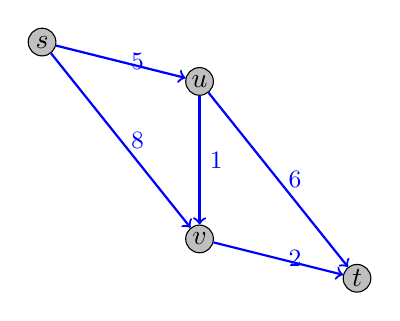
\begin{tikzpicture}[scale=1., auto,swap]
    % Draw a 7,11 network
    % First we draw the vertices
    \foreach \pos/\name in {{(0,1.5)/s}, {(2,1)/u}, {(2,-1)/v},
                            {(4,-1.5)/t}}
        \node[smallvertex] (\name) at \pos {$\name$};
    % Connect vertices with edges and draw weights
    \foreach \source/ \dest /\weight in {s/u/5, u/t/6,u/v/1,s/v/8,          v/t/2}
        \path[edge, blue] (\source) -- node[weight, right] {\small $\weight$} (\dest);

%    \foreach \source/ \dest /\weight in {s/u/{x_{1}}, u/t/{x_{4}},u/v/{x_{3}},s/v/{x_{2}},          v/t/{x_{5}}}
%        \path[edge, blue] (\source) -- node[weight, left] {$\weight$} (\dest);
%       \draw[dashed, ->] (0,0) arc  (120:60:2);
     \end{tikzpicture}
\end{figure}


\textbf{最短路径问题的对偶以及简化}

写出它的原始线性规划:
\begin{small}
\[
\begin{array}{rrrrrrrrrrll}
 \min &5 x_1   &+&  8 x_2   &+& 1 x_3   &+& 6 x_4   &+& 2 x_5 & \\
 s.t. & x_1 &+&  x_2 & &  & &   & & & = 1    & \text{vertex } s \\
      &     & &      & &  &-&   x_4  &-& x_5 & = -1 &\text{vertex } t  \\
      &  -x_1& &     &+& x_3 &+& x_4  & & & =  0  &\text{vertex } u \\
      &      &-& x_2 &-& x_3 & &      &+&x_5 & =  0 &\text{vertex } v  \\
      &   x_1 &,&     x_2 &,&    x_3  &,&    x_4  &,& x_5 & \textcolor{red}{\geq 0} \\
       &   x_1 &,&     x_2 &,&    x_3  &,&    x_4  &,& x_5 & \textcolor{red}{\leq 1} 	
\end{array} \nonumber
\]
\end{small}
对于约束条件,我们要求xi应该取0或者1。如果这样的话,问题挺难的。对于这个问题,我们可以松弛一下,变成大于等于0小于等于1.由于全单模条件,这两个条件的解是一样的。

写出原问题的对偶:
\begin{small}
\[
\begin{array}{rrrrrrrrrl}
 \max & y_s   &-& y_t  \\
 s.t. & y_s & &      &-& y_u & &     &  \leq 5 & \textcolor{blue}{x_{1}: \text{edge } (s,u)}  \\
      & y_s & &      & &     &-& y_v &  \leq 8 & \textcolor{blue}{x_{2}: \text{edge } (s,v)}   \\
      &     & &      & & y_u &-& y_v &  \leq 1 & \textcolor{blue}{x_{3}: \text{edge } (u,v)}  \\
      &     &-& y_t  & + & y_u & &     &  \leq 6 & \textcolor{blue}{x_{4}: \text{edge } (u,t)}  \\
      &     &-& y_t  & &     &+& y_v &  \leq 2 & \textcolor{blue}{x_{5}: \text{edge } (v,t)}  \\
\end{array} \nonumber
\]
\end{small}
原问题相当于对每个边设一个变量,对偶问题相当于对城市设置变量。yi可以理解为城市i的海拔高度。优化目标为ys-yt,是原问题的下边界。求它的最大值。
\begin{figure}[H]
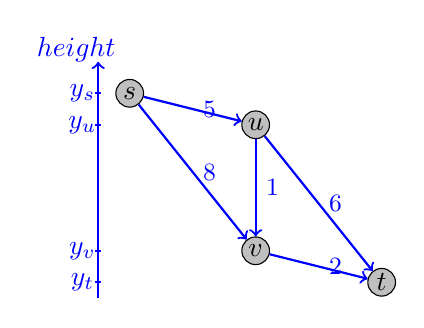
\begin{tikzpicture}[scale=0.8, auto,swap]
    % Draw a 7,11 network
    % First we draw the vertices
    \foreach \pos/\name in {{(0,1.5)/s}, {(2,1)/u}, {(2,-1)/v},
                            {(4,-1.5)/t}}
        \node[smallvertex] (\name) at \pos {$\name$};
    % Connect vertices with edges and draw weights
    \foreach \source/ \dest /\weight in {s/u/5, u/t/6,u/v/1,s/v/8,          v/t/2}
        \path[edge, blue] (\source) -- node[weight, right] {\small $\weight$} (\dest);

%    \foreach \source/ \dest /\weight in {s/u/{x_{1}}, u/t/{x_{4}},u/v/{x_{3}},s/v/{x_{2}},          v/t/{x_{5}}}
%        \path[edge, blue] (\source) -- node[weight, left] {$\small  \weight$} (\dest);

%       \draw[dashed, ->] (0,0) arc  (120:60:2);
   \draw[->, blue, thick] (-0.5, -1.75) -- (-0.5, 2);
   \node[blue] at (-0.85, 2.2) {$height$};
   \foreach \y/\name in {-1.5/t, -1/v, 1/u, 1.5/s}
   {
   	\draw[blue, thick] (-0.55, \y) -- (-0.45, \y);
	\node[blue]  at (-0.75, \y) {$y_\name$};
   }
   \end{tikzpicture}
\end{figure}

跑原始对偶算法,首先简化原始问题,将yt固定为0。问题变为:
\begin{small}
\[
\begin{array}{rrrrrrrrrl}
 \max & y_s   & &   \\
 s.t. & y_s & &      &-& y_u & &     &  \leq 5 & \textcolor{blue}{x_{1}: \text{edge } (s,u)}  \\
      & y_s & &      & &     &-& y_v &  \leq 8 & \textcolor{blue}{x_{2}: \text{edge } (s,v)}   \\
      &     & &      & & y_u &-& y_v &  \leq 1 & \textcolor{blue}{x_{3}: \text{edge } (u,v)}  \\
      &     & &    &   & y_u & &     &  \leq 6 & \textcolor{blue}{x_{4}: \text{edge } (u,t)}  \\
      &     & &   & &     & & y_v &  \leq 2 & \textcolor{blue}{x_{5}: \text{edge } (v,t) } \\
\end{array} \nonumber
\]
\end{small}


\textbf{第一次迭代}

设置一个初始可行解: $\mathbf{y^T} = (0, 0, 0)$.将其带入约束,判断哪些约束取等号,哪些取不等。根据互补松弛性,确定哪些xi=0。
 \begin{small}
\[
\begin{array}{rrrrrrrrrrl}
 & y_s & &      &-& y_u & &     &  \textcolor{blue}{<}& 5 &  \textcolor{blue}{\Rightarrow  x_{1}  = 0}   \\
 & y_s & &      & &     &-& y_v &   \textcolor{blue}{<}&  8 & \textcolor{blue}{\Rightarrow  x_{2}  = 0}  \\
  &     & &      & & y_u &-& y_v &   \textcolor{blue}{<}&  1 & \textcolor{blue}{\Rightarrow  x_{3}  = 0} \\
 &     & &    &   & y_u & &     &   \textcolor{blue}{<}&  6 & \textcolor{blue}{\Rightarrow  x_{4}  = 0}  \\
 &     & &   & &     & & y_v &   \textcolor{blue}{<}&  2 & \textcolor{blue}{\Rightarrow  x_{5}  = 0}
\end{array} \nonumber
\]
\end{small}
验证可知在$D$中, \textcolor{red}{$J=\Phi$},即 $x_2,x_3,x_4,x_5=0$。

把当前的RP写出来:
\[
\begin{array}{rrrrrrrrrrrrrrrrrl}
 \min & s_1 &+s_2 & +s_3 &     &        &    &     &   & \\
 s.t. & s_1 &     &     & \textcolor{blue}{+x_1}  & \textcolor{blue}{+x_2} &    &     &   & = 1    & \text{node }s  \\
%       &     & &      & &  &-&   x_4  &-& x_5 & = -1 &\text{vertex t}  \\
     &      &s_2     &             &  \textcolor{blue}{-x_1}  &     & \textcolor{blue}{+x_3}  &  \textcolor{blue}{+x_4}     &  & =  0  & \text{node }u\\
     &      &          & s_3       &     & \textcolor{blue}{-x_2}    & \textcolor{blue}{-x_3}  &      & \textcolor{blue}{+x_5} & =  0 & \text{node }v \\
     & s_1, &s_2, &s_3,  &      &          &         &         &     & \geq 0 \\
     &         &       &         &  \textcolor{blue}{x_1,} &    \textcolor{blue}{ x_2,} &    \textcolor{blue}{x_3,} &   \textcolor{blue}{x_4,} & \textcolor{blue}{x_5} & \textcolor{blue}{= 0} \\ 	
\end{array} \nonumber
\]
蓝色的xi是为了突出表示xi=0。

写出DRP:
\[
\begin{array}{rrrrrrrrrl}
 \max & y_s &      & &            &\\
s.t. & y_s  &      & &     \leq 1 &  \\
     &      & y_u  & &     \leq 1 &  \\
     &      &      & & y_v \leq 1 &  \\
\end{array} \nonumber
\]
如果原先的$\mathbf{y}$(0,0,0)是最优解的话,对应的$x$一定满足RP, $\Delta \mathbf{y}$满足DRP.

原始对偶算法应用到图论上,常常是这样的:写出的线性规划,对应的DRP形式很特殊,解能够很明显的看出来。

采用组合技术求解$DRP$,通过DRP求解,可以知道当前的y不是最优。对于DRP的最优值,找一个最优解 $\Delta \mathbf{y^T} = (1, 0, 0)$。(最优解不唯一)

计算步长$\theta$: $\theta = \min \{ \frac{ \mathbf{c_1 - y^Ta_1} }{ \mathbf{\Delta y^T a_1}  }, \frac{ \mathbf{c_2 - y^Ta_2} }{ \mathbf{\Delta y^T a_2}  }  \} = \min\{ 5, 8\} = 5$

更新 $\mathbf{y}$: $\mathbf{y^T=y^T}+\theta \Delta \mathbf{y^T}  = (5, 0, 0)$.

经过一次迭代更新以后,城市之间的状态如图:
\begin{figure}[H]
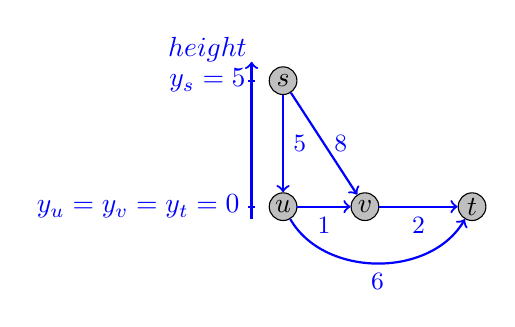
\begin{tikzpicture}[scale=0.8, auto,swap]

    \def\ys{2};
    \def\yu{0};
    \def\yv{0};
    \def\yt{0};

    \foreach \pos/\name in {{(0,\ys)/s}, {(0,\yu)/u}, {(1.3,\yv)/v}, {(3,\yt)/t}}
        \node[smallvertex] (\name) at \pos {$\name$};

    \foreach \source/ \dest /\weight in {s/u/5,s/v/8}
        \path[edge, blue] (\source) -- node[weight, right] {\small $\weight$} (\dest);
    \foreach \source/ \dest /\weight in { u/v/1, v/t/2}
        \path[edge, blue] (\source) -- node[weight, below] {\small $\weight$} (\dest);
    \draw[->, thick, blue] (u) to[out=-60, in=240] node[below]{\small $6$} (t);

   \draw[->, blue, thick] (-0.5, -0.2) -- (-0.5, 2.3);
   \node[blue] at (-1.2, 2.5) {$height$};

    	\draw[blue, thick] (-0.55, \yu) -- (-0.45, \yu);
	\node[blue]  at (-2.3, \yu) {$y_u=y_v=y_t=0$};

    	\draw[blue, thick] (-0.55, \ys) -- (-0.45, \ys);
	\node[blue]  at (-1.2, \ys) {$y_s=5$};

   \end{tikzpicture}
\end{figure}

我们就拿这一步来看,为什么说原始对偶算法就是Dijkstra's algorithm。

从Dijkstra's algorithm的角度来看:

DRP的最优解:$\Delta \mathbf{y^T} = (1, 0, 0)$,对应着Dijkstra's algorithm滴墨水的起始位置,也是被染的点集合$S = \{s\}$。第一次的最优解对应染的第一个点。DRP的实际目的找到墨水所要染的点。

步长 $\theta = \min \{ \frac{ \mathbf{c_1 - y^Ta_1} }{ \mathbf{\Delta y^T a_1}  }, \frac{ \mathbf{c_2 - y^Ta_2} }{ \mathbf{\Delta y^T a_2}  }  \} = \min\{ 5, 8\} = 5$:对于现在墨水所染得点集合 $S$ ,下一次墨水能染的最短距离。


\textbf{第二次迭代}

将新的可行解 $\mathbf{ y^T = (5, 0, 0) }$带入,检查约束:
 \begin{small}
\[
\begin{array}{rrrrrrrrrrl}
 & y_s & &      &-& y_u & &     &  \textcolor{red}{=}& 5 &  \\
 & y_s & &      & &     &-& y_v &   \textcolor{blue}{<}&  8 & \textcolor{blue}{\Rightarrow  x_{2}  = 0}  \\
  &     & &      & & y_u &-& y_v &   \textcolor{blue}{<}&  1 & \textcolor{blue}{\Rightarrow  x_{3}  = 0} \\
 &     & &    &   & y_u & &     &   \textcolor{blue}{<}&  6 & \textcolor{blue}{\Rightarrow  x_{4}  = 0}  \\
 &     & &   & &     & & y_v &   \textcolor{blue}{<}&  2 & \textcolor{blue}{\Rightarrow  x_{5}  = 0}
\end{array} \nonumber
\]
\end{small}
可知在$D$中:  \textcolor{red}{$J=\{ 1\}$}, 即 $x_2,x_3,x_4,x_5=0$.

对应的RP:
\[
\begin{array}{rrrrrrrrrrrrrrrrrl}
 \min & s_1 &+s_2 & +s_3 &     &        &    &     &   & \\
 s.t. & s_1 &     &     & \textcolor{blue}{+x_1}  & \textcolor{blue}{+x_2} &    &     &   & = 1    & \text{node }s  \\
%       &     & &      & &  &-&   x_4  &-& x_5 & = -1 &\text{vertex t}  \\
     &      &s_2     &             &  \textcolor{blue}{-x_1}  &     & \textcolor{blue}{+x_3}  &  \textcolor{blue}{+x_4}     &  & =  0  & \text{node }u\\
     &      &          & s_3       &     & \textcolor{blue}{-x_2}    & \textcolor{blue}{-x_3}  &      & \textcolor{blue}{+x_5} & =  0 & \text{node }v \\
     & s_1, &s_2, &s_3,  &      &          &         &         &     & \geq 0 \\
     &         &       &         &  \textcolor{blue}{x_1,} &    \textcolor{blue}{ x_2,} &    \textcolor{blue}{x_3,} &   \textcolor{blue}{x_4,} & \textcolor{blue}{x_5} & \textcolor{blue}{= 0} \\ 	
\end{array} \nonumber
\]

写出DRP:
\[
\begin{array}{rrrrrrrrrl}
 \max & y_s &      & &            &\\
s.t. & y_s  &      & &     \leq 1 &  \\
     &      & y_u  & &     \leq 1 &  \\
     &      &      & & y_v \leq 1 &  \\
\end{array} \nonumber
\]

采用组合技术求解$DRP$,通过DRP求解,可以知道当前的y不是最优。对于DRP的最优值,找一个最优解 $\Delta \mathbf{y^T} = (1, 0, 0)$。(最优解不唯一)
步长$\theta$: $\theta = \min \{ \frac{ \mathbf{c_1 - y^Ta_1} }{ \mathbf{\Delta y^T a_1}  }, \frac{ \mathbf{c_2 - y^Ta_2} }{ \mathbf{\Delta y^T a_2}  }  \} = \min\{ 5, 8\} = 5$。

更新$\mathbf{y}$: $\mathbf{y^T=y^T}+\theta \Delta \mathbf{y^T}  = (5, 0, 0)$.

经过第二次迭代更新以后,城市之间的状态如图:
\begin{figure}[H]
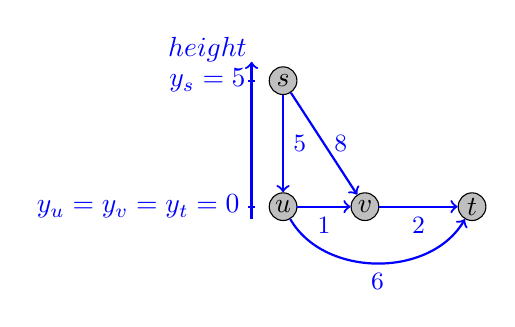
\begin{tikzpicture}[scale=0.8, auto,swap]

    \def\ys{2};
    \def\yu{0};
    \def\yv{0};
    \def\yt{0};

    \foreach \pos/\name in {{(0,\ys)/s}, {(0,\yu)/u}, {(1.3,\yv)/v}, {(3,\yt)/t}}
        \node[smallvertex] (\name) at \pos {$\name$};

    \foreach \source/ \dest /\weight in {s/u/5,s/v/8}
        \path[edge, blue] (\source) -- node[weight, right] {\small $\weight$} (\dest);
    \foreach \source/ \dest /\weight in { u/v/1, v/t/2}
        \path[edge, blue] (\source) -- node[weight, below] {\small $\weight$} (\dest);
    \draw[->, thick, blue] (u) to[out=-60, in=240] node[below]{\small $6$} (t);

   \draw[->, blue, thick] (-0.5, -0.2) -- (-0.5, 2.3);
   \node[blue] at (-1.2, 2.5) {$height$};

    	\draw[blue, thick] (-0.55, \yu) -- (-0.45, \yu);
	\node[blue]  at (-2.3, \yu) {$y_u=y_v=y_t=0$};

    	\draw[blue, thick] (-0.55, \ys) -- (-0.45, \ys);
	\node[blue]  at (-1.2, \ys) {$y_s=5$};

   \end{tikzpicture}
\end{figure}

从Dijkstra's algorithm的角度来看:

DRP的最优解:$\Delta \mathbf{y^T} = (1, 1, 0)$,对应着被染的点集合$S = \{s, u\}$ 。事实上,DRP的求解通过从$s$可达的节点中寻找确定。

步长  $\theta = \min \{
\frac{ \mathbf{c_2 - y^Ta_2} }{ \mathbf{\Delta y^T a_2}  },
\frac{ \mathbf{c_3 - y^Ta_3} }{ \mathbf{\Delta y^T a_3}  },
\frac{ \mathbf{c_4 - y^Ta_4} }{ \mathbf{\Delta y^T a_4}  }
\} = \min\{ 3, 1, 6\} = 1$:对于现在墨水所染得点集合 $S$ ,下一次墨水能染的最短距离。


\textbf{第三次迭代}

将新的可行解 $\mathbf{ y^T = (6, 1, 0) }$.带入,检查约束:
\begin{small}
\[
\begin{array}{rrrrrrrrrrl}
 & y_s & &      &-& y_u & &     &  \textcolor{red}{=}& 5 &  \\
 & y_s & &      & &     &-& y_v &   \textcolor{blue}{<}&  8 & \textcolor{blue}{\Rightarrow  x_{2}  = 0}  \\
  &     & &      & & y_u &-& y_v &   \textcolor{red}{=}&  1 &  \\
 &     & &    &   & y_u & &     &   \textcolor{blue}{<}&  6 & \textcolor{blue}{\Rightarrow  x_{4}  = 0}  \\
 &     & &   & &     & & y_v &   \textcolor{blue}{<}&  2 & \textcolor{blue}{\Rightarrow  x_{5}  = 0}
\end{array} \nonumber
\]
\end{small}
可知在$D$中: \textcolor{red}{$J=\{ 1, 3\}$}, 即 $x_2,x_4,x_5=0$.

对应的RP:
\[
\begin{array}{rrrrrrrrrrrrrrrrrl}
 \min & s_1 &+s_2 & +s_3 &     &        &    &     &   & \\
 s.t. & s_1 &     &     & \textcolor{red}{+x_1}  & \textcolor{blue}{+x_2} &    &     &   & = 1    & \text{node }s  \\
%       &     & &      & &  &-&   x_4  &-& x_5 & = -1 &\text{vertex t}  \\
     &      &s_2     &             &  \textcolor{red}{-x_1}  &     & \textcolor{red}{+x_3}  &  \textcolor{blue}{+x_4}     &  & =  0  & \text{node }u\\
     &      &          & s_3       &     & \textcolor{blue}{-x_2}    & \textcolor{red}{-x_3}  &      & \textcolor{blue}{+x_5} & =  0 & \text{node }v \\
     & s_1, &s_2, &s_3,  &      &          &         &         &     & \geq 0 \\
     &         &       &         &    &    \textcolor{blue}{ x_2,} &      &   \textcolor{blue}{x_4,} & \textcolor{blue}{x_5} & \textcolor{blue}{= 0} \\ 	
\end{array} \nonumber
\]

写出DRP:
\[
\begin{array}{rrrrrrrrrl}
 \max & y_s   & &    \\
 s.t. & y_s &-& y_u  & &     &  \leq 0 &  \\
     &  & &   y_u   &-& y_v &  \leq 0 & \\
      & y_s &,& y_u  &,& y_v &  \leq 1 &  \\
\end{array} \nonumber
\]

采用组合技术求解$DRP$,通过DRP求解,可以知道当前的y不是最优。对于DRP的最优值,找一个最优解  $\Delta \mathbf{y^T} = (1, 1, 1)$。(最优解不唯一)
步长$\theta$: $\theta = \min \{
\frac{ \mathbf{c_4 - y^Ta_4} }{ \mathbf{\Delta y^T a_4}  } ,
\frac{ \mathbf{c_5 - y^Ta_5} }{ \mathbf{\Delta y^T a_5}  }
\} = \min\{ 5, 2 \} = 2$。

更新$\mathbf{y}$: $\mathbf{y^T=y^T}+\theta \Delta \mathbf{y^T}  = (8, 3, 2)$..

经过第三次迭代更新以后,城市之间的状态如图:
\begin{figure}[H]
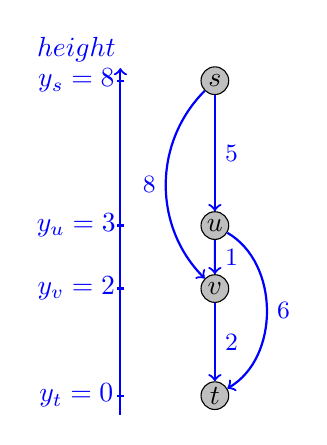
\begin{tikzpicture}[scale=0.8, auto,swap]

    \def\ys{3.3};
    \def\yu{1};
    \def\yv{0};
    \def\yt{-1.7};

    \foreach \pos/\name in {{(1,\ys)/s}, {(1,\yu)/u}, {(1,\yv)/v}, {(1,\yt)/t}}
        \node[smallvertex] (\name) at \pos {$\name$};

    \foreach \source/ \dest /\weight in {s/u/5,u/v/1}
        \path[edge, blue] (\source) -- node[weight, right] {\small $\weight$} (\dest);
    \foreach \source/ \dest /\weight in {  v/t/2}
        \path[edge, blue] (\source) -- node[weight, right] {\small $\weight$} (\dest);
    \draw[->, thick, blue] (u) to[out=-30, in=30] node[right]{\small $6$} (t);
    \draw[->, thick, blue] (s) to[out=225, in=135] node[left]{\small $8$} (v);

   \draw[->, blue, thick] (-0.5, -2) -- (-0.5, 3.5);
   \node[blue] at (-1.2, 3.8) {$height$};

    	\draw[blue, thick] (-0.55, \yv) -- (-0.45, \yv);
	\node[blue]  at (-1.2, \yv) {$y_v=2$};
	
    	\draw[blue, thick] (-0.55, \yt) -- (-0.45, \yt);
	\node[blue]  at (-1.2, \yt) {$y_t=0$};

    	\draw[blue, thick] (-0.55, \ys) -- (-0.45, \ys);
	\node[blue]  at (-1.2, \ys) {$y_s=8$};

    	\draw[blue, thick] (-0.55, \yu) -- (-0.45, \yu);
	\node[blue]  at (-1.2, \yu) {$y_u=3$};	

   \end{tikzpicture}
\end{figure}

从Dijkstra's algorithm的角度来看:

DRP的最优解: $\Delta \mathbf{y^T} = (1, 1, 1)$,对应着被染的点集合$S = \{s, u, v\}$。事实上,DRP的求解通过从$s$可达的节点中寻找确定。

步长$\theta = \min \{
\frac{ \mathbf{c_4 - y^Ta_4} }{ \mathbf{\Delta y^T a_4}  } ,
\frac{ \mathbf{c_5 - y^Ta_5} }{ \mathbf{\Delta y^T a_5}  }
\} = \min\{ 5, 2 \} = 2$:对于现在墨水所染得点集合 $S$ ,下一次墨水能染的最短距离。


\textbf{第四次迭代}

将新的可行解$\mathbf{ y^T = (8, 3, 2) }$.带入,检查约束:
\begin{small}
\[
\begin{array}{rrrrrrrrrrl}
 & y_s & &      &-& y_u & &     &  \textcolor{red}{=}& 5 &  \\
 & y_s & &      & &     &-& y_v &   \textcolor{blue}{<}&  8 & \textcolor{blue}{\Rightarrow  x_{2}  = 0}  \\
  &     & &      & & y_u &-& y_v &   \textcolor{red}{=}&  1 &  \\
 &     & &    &   & y_u & &     &   \textcolor{blue}{<}&  6 & \textcolor{blue}{\Rightarrow  x_{4}  = 0}  \\
 &     & &   & &     & & y_v &   \textcolor{red}{=}&  2 &
\end{array} \nonumber
\]
\end{small}
可知在$D$中: \textcolor{red}{$J=\{ 1, 3\}$}, 即 $x_2,x_4,x_5=0$.

对应的RP:
\[
\begin{array}{rrrrrrrrrrrrrrrrrl}
 \min & s_1 &+s_2 & +s_3 &     &        &    &     &   & \\
 s.t. & s_1 &     &     & \textcolor{red}{+x_1}  & \textcolor{blue}{+x_2} &    &     &   & = 1    & \text{node }s  \\
%       &     & &      & &  &-&   x_4  &-& x_5 & = -1 &\text{vertex t}  \\
     &      &s_2     &             &  \textcolor{red}{-x_1}  &     & \textcolor{red}{+x_3}  &  \textcolor{blue}{+x_4}     &  & =  0  & \text{node }u\\
     &      &          & s_3       &     & \textcolor{blue}{-x_2}    & \textcolor{red}{-x_3}  &      & \textcolor{red}{+x_5} & =  0 & \text{node }v \\
     & s_1, &s_2, &s_3,  &      &          &         &         &     & \geq 0 \\
     &         &       &         &    &    \textcolor{blue}{ x_2,} &      &   \textcolor{blue}{x_4} &  & \textcolor{blue}{= 0} \\ 	
\end{array} \nonumber
\]

写出DRP:
\[
\begin{array}{rrrrrrrrrl}
 \max & y_s   & &    \\
 s.t. & y_s &-& y_u  & &     &  \leq 0 &  \\
     &  & &   y_u   &-& y_v &  \leq 0 & \\
     &  & &       & & y_v &  \leq 0 & \\
      & y_s &,& y_u  &,& y_v &  \leq 1 &  \\
\end{array} \nonumber
\]

采用组合技术求解$\Delta \mathbf{y^T} = (0, 0, 0)$,可知当前时刻$y$为最优解。

经过第四次迭代更新以后,城市之间的状态如图:
\begin{figure}[H]
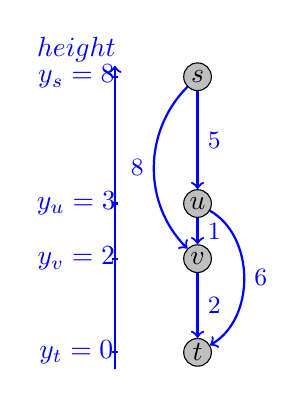
\begin{tikzpicture}[scale=0.7, auto,swap]

    \def\ys{3.3};
    \def\yu{1};
    \def\yv{0};
    \def\yt{-1.7};

    \foreach \pos/\name in {{(1,\ys)/s}, {(1,\yu)/u}, {(1,\yv)/v}, {(1,\yt)/t}}
        \node[smallvertex] (\name) at \pos {$\name$};

    \foreach \source/ \dest /\weight in {s/u/5,u/v/1}
        \path[edge, blue] (\source) -- node[weight, right] {\small $\weight$} (\dest);
    \foreach \source/ \dest /\weight in {  v/t/2}
        \path[edge, blue] (\source) -- node[weight, right] {\small $\weight$} (\dest);
    \draw[->, thick, blue] (u) to[out=-30, in=30] node[right]{\small $6$} (t);
    \draw[->, thick, blue] (s) to[out=225, in=135] node[left]{\small $8$} (v);

   \draw[->, blue, thick] (-0.5, -2) -- (-0.5, 3.5);
   \node[blue] at (-1.2, 3.8) {$height$};

    	\draw[blue, thick] (-0.55, \yv) -- (-0.45, \yv);
	\node[blue]  at (-1.2, \yv) {$y_v=2$};
	
    	\draw[blue, thick] (-0.55, \yt) -- (-0.45, \yt);
	\node[blue]  at (-1.2, \yt) {$y_t=0$};

    	\draw[blue, thick] (-0.55, \ys) -- (-0.45, \ys);
	\node[blue]  at (-1.2, \ys) {$y_s=8$};

    	\draw[blue, thick] (-0.55, \yu) -- (-0.45, \yu);
	\node[blue]  at (-1.2, \yu) {$y_u=3$};	

   \end{tikzpicture}
\end{figure}

从Dijkstra's algorithm的角度来看:

DRP的最优解: $\Delta \mathbf{y^T} = (0, 0, 0)$,表示能找到一个路径path从s到t,强迫$y_{s} = 0$  。这对应Dijkstra's algorithm中那滴墨水把所有的点都染到了。

Dijkstra's algorithm的另一个直观解释为:用一些绳子连着一些球,拎起s点,然后让t点在最下面,求两者最短距离。

原始算法十分重要,希望大家好好掌握
\section{网络流及其应用1}
\subsection{概述}
我们来讲网络流问题:
\begin{itemize}
\item {\sc MaximumFlow} problem: {\sc Ford-Fulkerson} algorithm, {\sc MaxFlow-MinCut} theorem;
\item A duality explanation of {\sc Ford-Fulkerson} algorithm and {\sc MaxFlow-MinCut} theorem(实际上就是强对偶性);
\item Scaling technique to improve {\sc Ford-Fulkerson} algorithm(值得大家学习);
\item Solving the dual problem: Push-Relabel algorithm;
%\item Connection with divide-and-conquer technique;
\item Extensions of {\sc MaximumFlow} problem: lower bound of capacity, multiple sources $\&$ multiple sinks, indirect graph;
%\item Applications of network flow: {\sc BipartiteMatching}, {\sc ProteinDomainParsing}, {\sc BaseballElimination}, {\sc ImageSegmentation}, {\sc SurveyDesign}, {\sc FlightScheduling};
\end{itemize}
\subsection{网络流的简短历史}

\begin{figure}[H]
 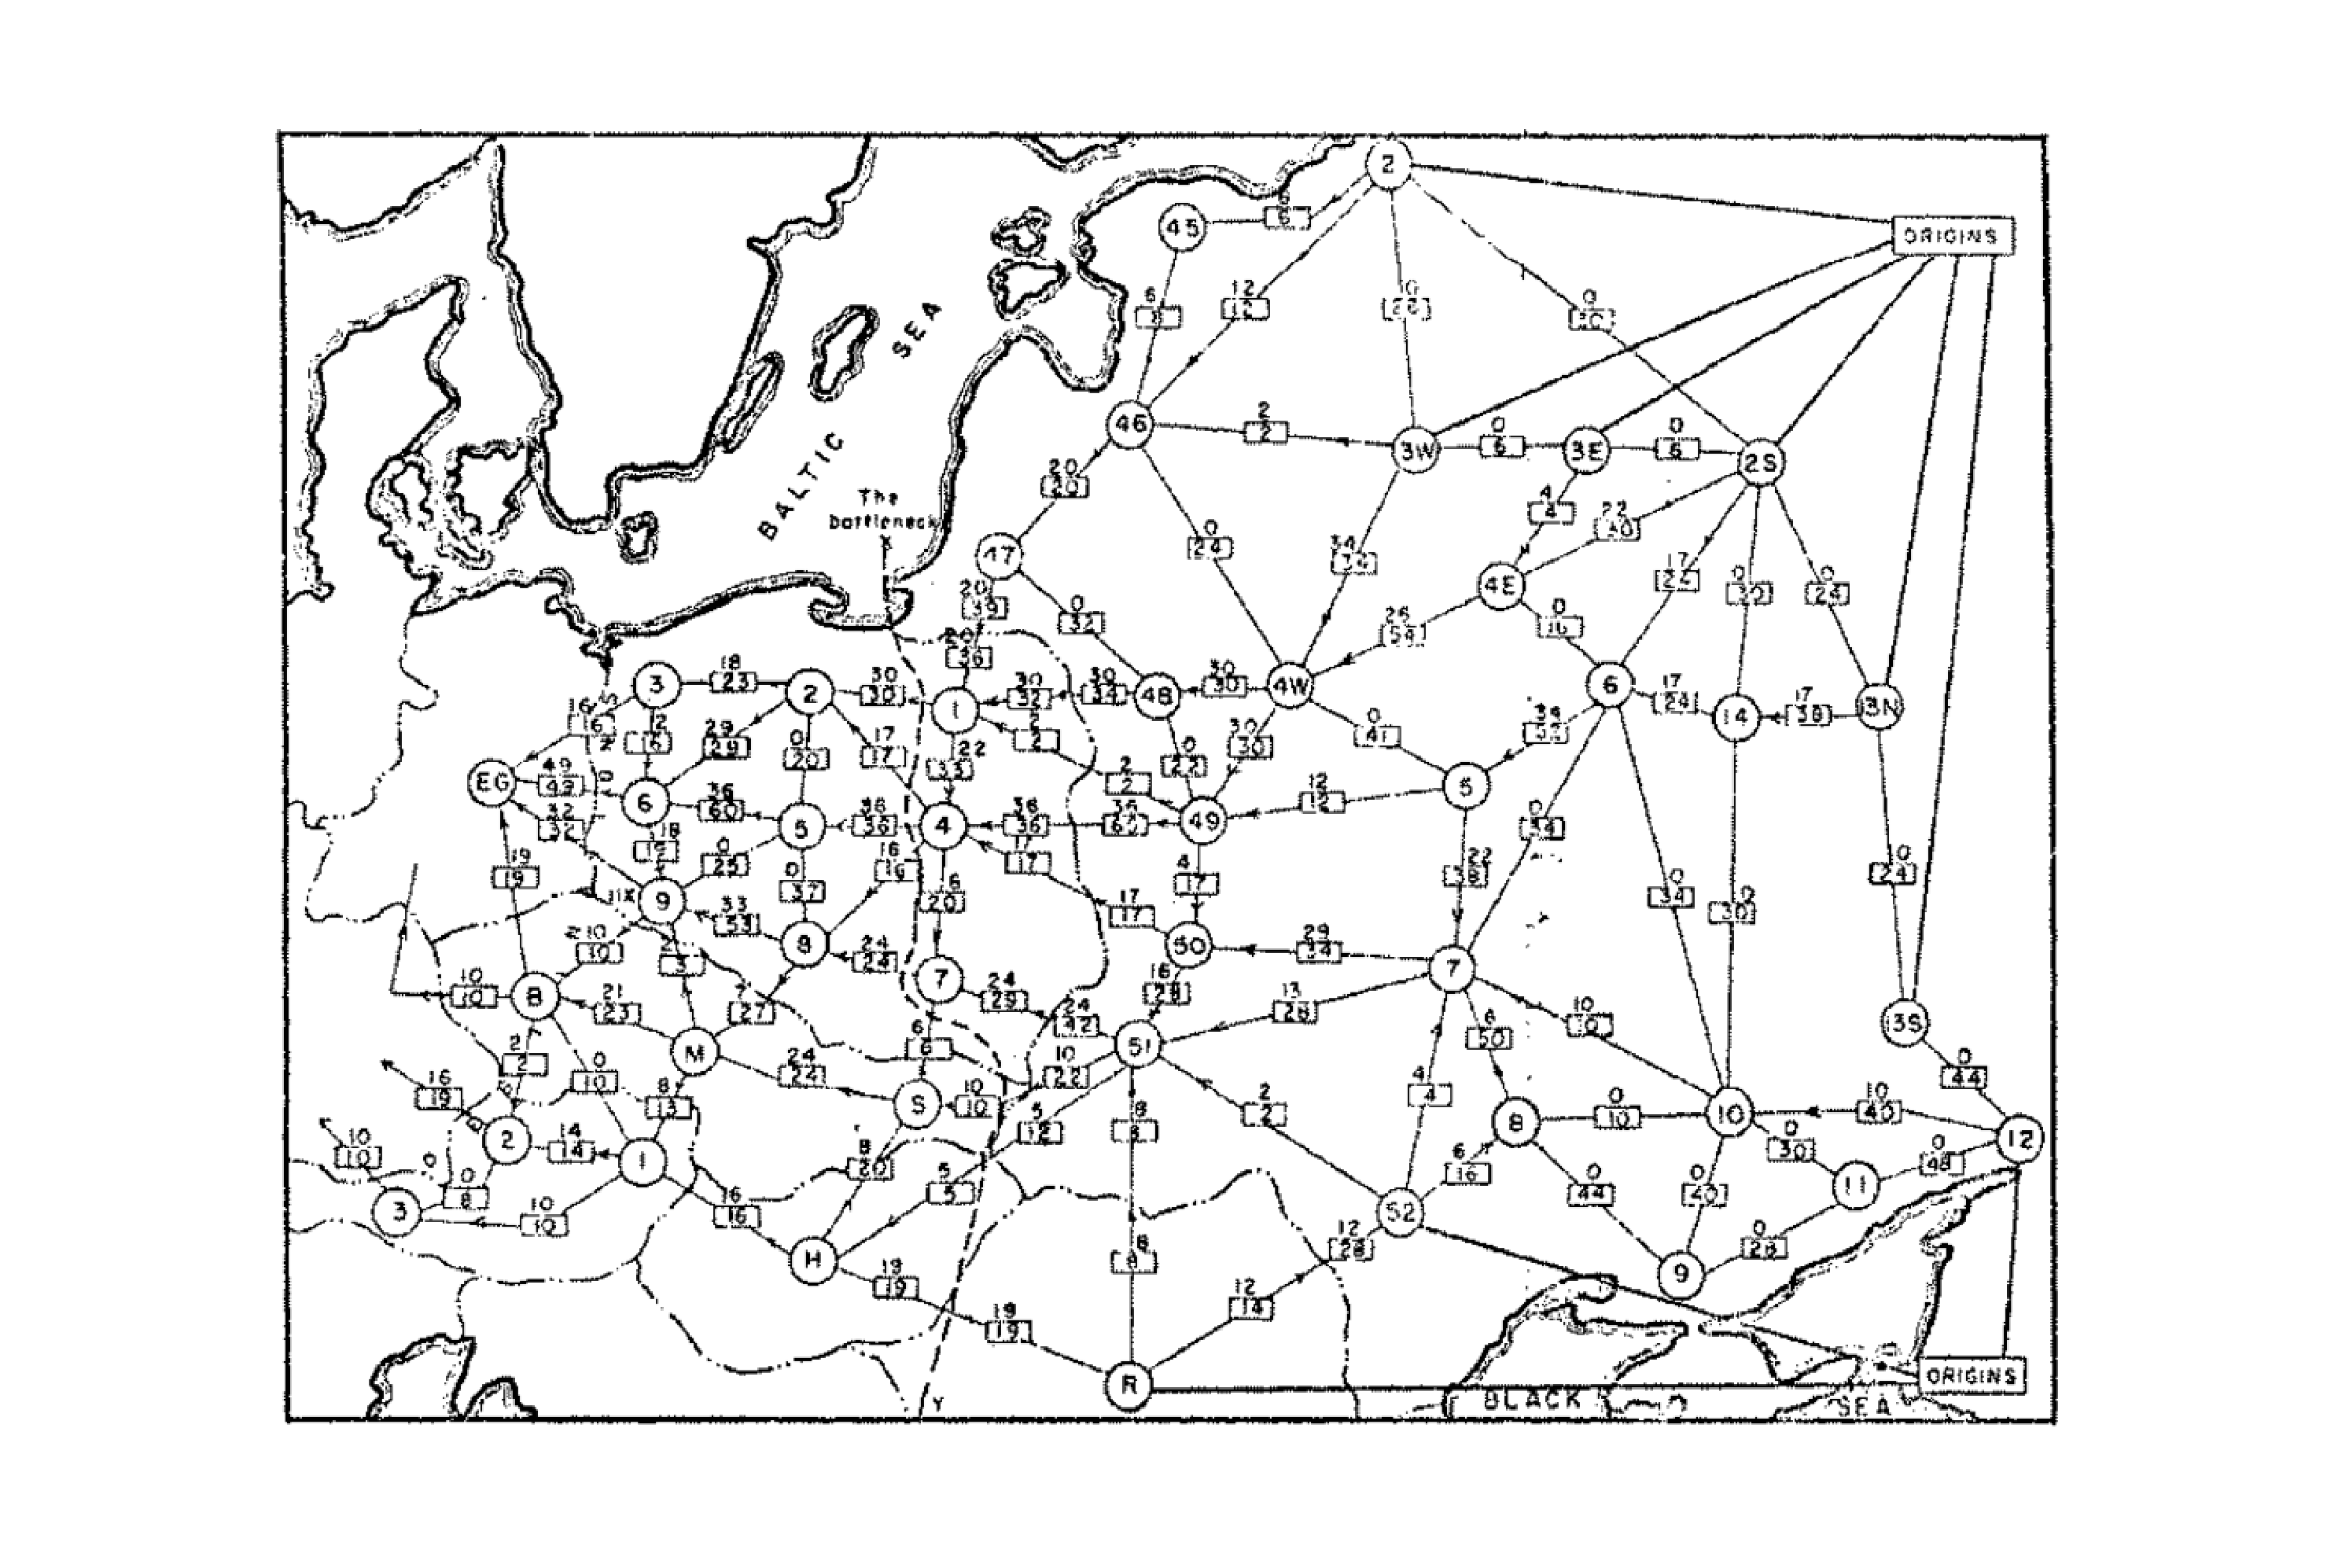
\includegraphics[width=3.5in] {L10-sovietunion.eps}
 \caption{Soviet Railway network, 1955}
\end{figure}
…… 1955年,美国开始在想,如何轰炸铁路,来阻断苏联同社会主义国家之间的联系。……
\begin{itemize}
 \item
\textit{``.... From Harris and Ross [1955]: Schematic diagram of the railway network of the Western
Soviet Union and Eastern European countries, with a maximum flow of value 163,000 tons
from Russia to Eastern Europe, and a cut of capacity 163,000 tons indicated as “The
bottleneck”. ....''}

\item
\textit{A recently declassified U.S. Air Force report indicates that the original motivation of minimum-cut problem and Ford-Fulkerson algorithm is \textcolor{red}{ to disrupt rail transportation the Soviet Union} [A. Shrijver, 2002].(2002年的解密文档) }
\end{itemize}
1955年提出的问题,到了1956年,Ford and Fulkerson就给了一个算法。从这个事情中又能够体现着出这件事情:原始问题的实际问题是什么,数学的抽象-建模是第二部,第三步是算法设计。

\begin{table}[H]
   {\begin{tabular}{lcc}\hline
%        & \multicolumn{3}{c}{Actual number of DCJ operations}\\
        Year  & Developers &  Time-complexity  \\
\hline
1956 & Ford and Fulkerson & $O(m C)$ and $O(m^2\log C)$ \\
1972 & Edmonds and Karp & $O(m^2 n)$ \\
1970 & Dinitz & $O(n^2 m)$ \\
1974 & Karzanov & $O(n^3)$ \\
1983 & Sleator and Tarjan & $O(nm \log n)$ \\
1988 & Goldberg and Tarjan & $O(n^2 m \log(\frac{n^{2}}{m}))$ \\
2012  & Orlin	& $O(nm)$ \\ \hline

     \end{tabular}} {}%
 \end{table}
\subsection{最大流问题}


\textbf{问题描述}
\begin{itemize}

\item 输入:
  一个有向图 $G=<V, E>$.每个顶点v表示一个城市,每条边e表示城市之间的路,每条边$e$有个容量限制$C_e$. 两个特殊的点:起点\textcolor{red}{\bf source} $s$ 和终点 \textcolor{red}{\bf sink} $t$;
\item 输出:
 对于每一条边 $e=(u, v)$, 分给一条流$f(u, v)$ 最终使得$\sum_{u, (s,u)\in E} f{(s,u)}$ 最大.
\end{itemize}

具体举例如下:
\begin{figure}[H]
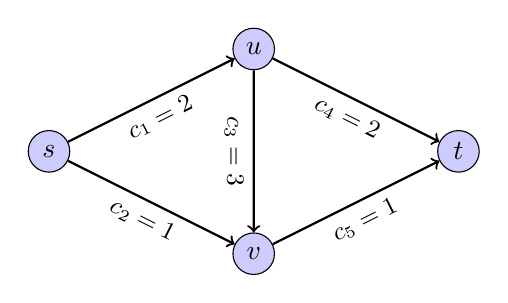
\begin{tikzpicture}[scale=1.3, auto,swap]
    % Draw a 7,11 network
    % First we draw the vertices
    \foreach \pos/\name in {{(0,0)/s}, {(2,1)/u}, {(2,-1)/v},
                            {(4,0)/t}}
        \node[middlevertex, draw,  fill=blue!20] (\name) at \pos {$\name$};
    % Connect vertices with edges and draw weights
    \foreach \source/ \dest /\weight in {s/u/{c_1=2}, u/t/{ c_4=2},u/v/{c_3=3},s/v/{c_2=1},      v/t/{c_5=1} }
        \path[edge, sloped, midway, below, allow upside down] (\source) -- node[weight] {$\weight$} (\dest);
   \end{tikzpicture}
\end{figure}
目标:从s点运尽量多的货物到目的地t。

\begin{figure}[H]
\begin{tikzpicture}[scale=1.3, auto,swap]
    % Draw a 7,11 network
    % First we draw the vertices
    % Connect vertices with edges and draw weights
    \foreach \source/ \dest /\weight in {s/u/{1/2}, u/t/{ 0/2},u/v/{1/3},s/v/{0/1},      v/t/{1/1} }
        \path[edge, sloped, midway, below, allow upside down] (\source) -- node[weight] {$\weight$} (\dest);
    \path[draw, thick, ->, blue] (0, 0) -- (2,1);
         \path[draw, thick, ->, blue] (2,1) -- (2,-1);
             \path[draw, thick, ->, blue] (2, -1) -- (4, 0);
    \foreach \pos/\name in {{(0,0)/s}, {(2,1)/u}, {(2,-1)/v},
                            {(4,0)/t}}
        \node[middlevertex, draw,  fill=blue!20] (\name) at \pos {$\name$};

   \end{tikzpicture}
\end{figure}


\textbf{定义:flow}

$f: E\rightarrow R^+$ 是一个 \textcolor{red}{\bf $s-t$ flow} 如果:
\begin{enumerate}
 \item   (Capacity constraints): $0\leq f(e) \leq C_e$ 对于全部的 $e$成立;
 \item   (Conservation constraints): 对于任何中间节点$v \in V-\{s,t\}$, $f^{in}(v) = f^{out}(v)$, 其中 $f^{in}(v) = \sum_{e \text{  into } v} f(e) $ 并且 $f^{out}(v) = \sum_{ e \text{ out of } v} f(e)$. (直观: 输入 = 输出 对于任何节点.)
\end{enumerate}
 \textcolor{red}{\bf flow 的值 $f$}被定义为 $V(f) = f^{out}(s)$.


\textbf{定义:$s-t$ cut}

一个 \textcolor{red} {\bf $s-t$ cut}是一个划分 $V$ 的$(A,B)$ 从而使得 $s\in A$ and $t \in B$.
\textcolor{red}{\bf 割 cut $(A,B)$的capacity} 被定义为 $C(A,B) = \sum_{e \text{ from } A \text{ to } B} C(e)$.

\begin{figure}[H]
\begin{tikzpicture}[scale=1.3, auto,swap]
    % Draw a 7,11 network
    % First we draw the vertices

    % Connect vertices with edges and draw weights
    \foreach \source/ \dest /\weight in {s/u/{c_1=2}, u/t/{ c_4=2},u/v/{c_3=3},s/v/{c_2=1},      v/t/{c_5=1} }
        \path[edge, sloped, midway, below, allow upside down] (\source) -- node[weight] {$\weight$} (\dest);

        \path[draw, thick, white, ->] (0,0)--(2,1);
        \path[draw, thick, white, ->] (2,-1)--(4,0);
        \path[draw, thick, green, ->] (0,0)--(2,1);
        \path[draw, thick, green, ->] (2,-1)--(4,0);
         \node[below, red] at (0, -0.5) {$\mathbf{A}$};
         \node[above, red] at (4, 0.5) {$\mathbf{B}$};
         \path[draw, thick, dashed, red] (0.5,0.75)--(3.5,-0.75);
            \foreach \pos/\name in {{(0,0)/s}, {(2,1)/u}, {(2,-1)/v},{(4,0)/t}}
        \node[middlevertex, draw,  fill=blue!20] (\name) at \pos {$\name$};

   \end{tikzpicture}
\end{figure}
\begin{center}
$C(A, B) = 3$,只计从A到B的,不计从B到A的
\end{center}

\textbf{定义:流值引理}

给定一个流  $f$. 对于 \textcolor{red}{\bf 任何}  $s-t$ 割 cut $(A,B)$, 通过这个割的流是一个常量$V(f)$. 通常,  $V(f) = f^{out}( A ) - f^{in} (A)$.

\begin{figure}[H]
\begin{tikzpicture}[scale=1.3, auto,swap]
    % Draw a 7,11 network
    % First we draw the vertices

    % Connect vertices with edges and draw weights
    \foreach \source/ \dest /\weight in {s/u/{2/2}, u/t/{ 1/2},u/v/{1/3},s/v/{0/1},      v/t/{1/1} }
        \path[edge, sloped, midway, below, allow upside down] (\source) -- node[weight] {$\weight$} (\dest);

        \path[draw, thick, green, ->] (0,0)--(2,1);
        \path[draw, thick, green, ->] (2,-1)--(4,0);
        \path[draw, thick, blue, ->] (2,1)--(2,-1);
        \path[draw, thick, dashed, red] (0.5, 0.5)--(0.5, -0.6);
         \node[below, red] at (0, -0.5) {$\mathbf{A}$};
         \node[above, red] at (4, 0.5) {$\mathbf{B}$};
         \path[draw, thick, dashed, red] (0.5,0.75)--(3.5,-0.75);
            \foreach \pos/\name in {{(0,0)/s}, {(2,1)/u}, {(2,-1)/v},{(4,0)/t}}
        \node[middlevertex, draw,  fill=blue!20] (\name) at \pos {$\name$};

   \end{tikzpicture}
\end{figure}
\begin{center}
$V(f) = 2 + 0 = 2$\\
$f^{out}(A) - f^{in}(A) = 2 + 1 - 1 = V(f)$
\end{center}

\begin{figure}[H]
\begin{tikzpicture}[scale=1.3]
    % Draw a 7,11 network
    % First we draw the vertices

    % Connect vertices with edges and draw weights
    \foreach \source/ \dest /\weight in {s/u/{2/2}, u/t/{ 1/2},u/v/{1/3},s/v/{0/1},      v/t/{1/1} }
        \path[edge, sloped, midway, below, allow upside down] (\source) -- node[weight] {$\weight$} (\dest);
        \path[draw, thick, green, ->] (0,0)--(2,1);
        \path[draw, thick, green, ->] (2,-1)--(4,0);
        \path[draw, thick, blue, ->] (2,1)--(2,-1);
         \node[below, red] at (0, -0.5) {$\mathbf{A}$};
         \node[above, red] at (4, 0.5) {$\mathbf{B}$};
         \path[draw, thick, dashed, red] (0.5,0.75)--(3.5,-0.75);
                 \path[draw, thick, dashed, red] (0.5, 0.5)--(0.5, -0.6);
            \foreach \pos/\name in {{(0,0)/s}, {(2,1)/u}, {(2,-1)/v},{(4,0)/t}}
        \node[middlevertex, draw,  fill=blue!20] (\name) at \pos {$\name$};
   \end{tikzpicture}
\end{figure}

\textbf{引理证明}
\begin{small}
\begin{itemize}
\item  我们有: $0 = f^{out}(v) - f^{in}(v) $ 对于任何的 $v \neq s$ 和 $v \neq t$.这是条件。
\item  因此我们有:
\begin{eqnarray}
V(f) &=& f^{out}(s) - f^{in} (s)  \text{\qquad\qquad//提示: } f^{in}(s) = 0;\nonumber \\
     &=&  \sum\nolimits_{v \in A} ( f^{out}(v) - f^{in}(v) ) \nonumber \\
     &=&\ ( \sum\nolimits_{\text{ e from A to B}} f(e) + \sum\nolimits_{\text{ e from A to A}} f(e) )  \nonumber \\
     & &-( \sum\nolimits_{\text{ e from B to  A}} f(e) + \sum\nolimits_{\text{ e  from A to A }} f(e) ) \nonumber \\
     &=&  f^{out}(A) - f^{in} (A) \nonumber
\end{eqnarray}
\end{itemize}
\end{small}

以上是一些定义和引理。现在回到原问题。依据我们现在所学的知识,采用什么方法使得流最大。贪心可以,但肯定不太好,分支特别多,不是一个太好的选择。线性规划肯定可以,是万能的。首先这个问题不好分,是图的问题,不好规约。下面看一下1956年的Ford-Fulkerson algorithm 。

\subsection{Ford-Fulkerson algorithm}

\textbf{Lester Randolph Ford Jr. 和 Delbert Ray Fulkerson}

 \begin{figure}[H]%
   \begin{center}%
     \begin{minipage}{0.40\textwidth}%
      \includegraphics[width=1.0\textwidth]{FordJr.png}%
     \end{minipage}%
     \qquad
     \begin{minipage}{0.40\textwidth}
      \includegraphics[width=1.0\textwidth]{Fulkerson.png}%
     \end{minipage}%
   \end{center}
   \caption{ Lester Randolph Ford Jr. and Delbert Ray Fulkerson}
 \end{figure}

\textbf{尝试1:动态规划技术}

\begin{itemize}
\item
动态规划似乎不太好用.
\item
实际上,当前不存在一个{\sc 最大流} 问题可以真正的被看做是属于动态规划问题.
 \item
我们知道 {\sc 最大流} 问题 是在 $\mathbf{P}$ 中因为它可以写成动态规划 (见 Lecture 8).
\item
然而, 网络结构存在它自己的属性使得能够有一个更有效的算法,非正式的称作 \textcolor{red}{\bf network simplex}, 等等.
\end{itemize}

\textbf{尝试2:{\sc 改进} 策略}

问题不好分,我们尝试改进的策略。


{\sc Improvement}$(f)$
\begin{algorithmic}[1]
\STATE $\mathbf{x=x_0}$; //starting from an initial solution;
\WHILE{ \texttt{TRUE} }
\STATE $\mathbf{x}=${\sc Improve}$(\mathbf{x})$; //move one step towards optimum;
\IF { {\sc Stopping}$(\mathbf{x, f})$ }
\STATE break;
\ENDIF
\ENDWHILE
\RETURN $\mathbf{x}$;
\end{algorithmic}


\textbf{迭代框架的三个关键问题}


三个问题:
\begin{enumerate}
\item 如何构建一个初始解?
	\begin{itemize}
	\item 对于 {\sc 最大流} 问题,  一个0-流可以通过通过设置$f(e)=0$得到,对于任意$e$.
	\item 很容验证h {\sc conservation} 和 {\sc capacity} 约束都被满足,对于0-流来说.
	\end{itemize}
\item 如何改进这个解决办法?
\item 何时停止?
\end{enumerate}

先看一个随便一想就能想到的办法。

 \begin{itemize}
 \item
假定$p$ 是一个在网络 $G$中的简单 ${s-t}$ path.

  \begin{algorithmic}[1]
    \STATE Initialize $f(e)=0$ for all $e$.
    \WHILE{there is an  $s-t$ path  in graph $G$}
    \STATE  \textcolor{red}{\bf arbitrarily} choose an $s-t$ path $p$ in $G$;
    \STATE $f = ${\sc augment}$(p, f)$;
    \ENDWHILE
    \RETURN{$f$};
  \end{algorithmic}
\end{itemize}

我们定义 $bottleneck(p, f)$ 作为 path $p$上边的最小capacity.

{\sc augment}$(p, f):$\\
  \begin{algorithmic}[1]
  \STATE Let $b=bottleneck(p, f);$
    \FOR{each edge $e=(u,v)$ $\in P$}
    \IF{$(u,v)$ is a forward edge}
    \STATE increase $f(u,v)$ by $b;$
    \ELSE
    \STATE decrease $f(u,v)$ by $b;$
    \ENDIF
    \ENDFOR
  \end{algorithmic}

这是一个失败的算法。\\

为什么会失败呢?

\begin{itemize}
 \item
我们从 0-流开始.
为了减小 $f$的值, 我们找到一条 $s-t$ path, 比如说 $p = s\rightarrow u  \rightarrow v$, 来运更多的商品
\item
这三条边上的流可以被增加$1$ 同时满足conservation和capacity限制.
\item
然而,我们不能发现一条$s-t$ path存在于 $G$ 中,使得 $f$ 增加更多(左半部分)即使最大流是$2$ (右半部分).

\end{itemize}


\begin{figure}[H]
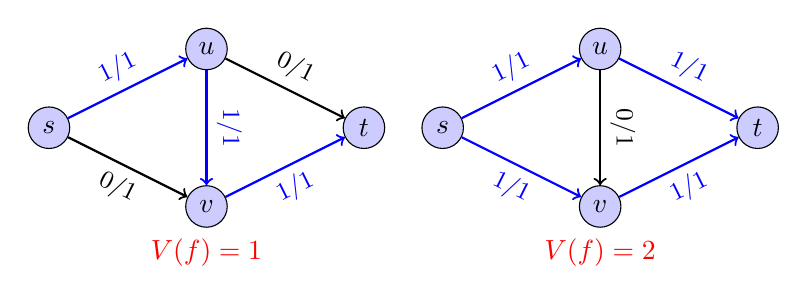
\begin{tikzpicture}[scale=1, auto,swap]

    \def\dx{0};
    \def\dy{0};	

     \foreach \x/\y/\name in { 0/0/s, 2/1/u, 2/-1/v, 4/0/t}
        \node[middlevertex, draw,  fill=blue!20] (\name) at (\x+\dx, \y+\dy) {$\name$};


    \foreach \source/ \dest /\weight in {s/u/{1/1}}
        \path[edge, sloped, midway, above, allow upside down, blue] (\source) -- node[weight] {\small $\weight$} (\dest);

    \foreach \source/ \dest /\weight in {u/t/{0/1}}
        \path[edge, sloped, midway, above, allow upside down] (\source) -- node[weight] {\small $\weight$} (\dest);

    \foreach \source/ \dest /\weight in {u/v/{1/1}}
        \path[edge, sloped, midway, above, allow upside down, blue] (\source) -- node[weight] {\small $\weight$} (\dest);

    \foreach \source/ \dest /\weight in {v/t/{1/1}}
        \path[edge, sloped, midway, below, allow upside down, blue] (\source) -- node[weight] {\small $\weight$} (\dest);

    \foreach \source/ \dest /\weight in {s/v/{0/1}}
        \path[edge, sloped, midway, below, allow upside down] (\source) -- node[weight] {\small $\weight$} (\dest);
       \node[ultra thick, red, below] at (v.south) {$V(f)=1$};


    \def\dx{5};
    \def\dy{0};	

     \foreach \x/\y/\name in { 0/0/s, 2/1/u, 2/-1/v, 4/0/t}
        \node[middlevertex, draw,  fill=blue!20] (\name) at (\x+\dx, \y+\dy) {$\name$};


    \foreach \source/ \dest /\weight in {s/u/{1/1}}
        \path[edge, sloped, midway, above, allow upside down, blue] (\source) -- node[weight] {\small $\weight$} (\dest);

    \foreach \source/ \dest /\weight in {u/t/{1/1}}
        \path[edge, sloped, midway, above, allow upside down, blue] (\source) -- node[weight] {\small $\weight$} (\dest);

    \foreach \source/ \dest /\weight in {u/v/{0/1}}
        \path[edge, sloped, midway, above, allow upside down ] (\source) -- node[weight] {\small $\weight$} (\dest);

    \foreach \source/ \dest /\weight in {v/t/{1/1}}
        \path[edge, sloped, midway, below, allow upside down, blue] (\source) -- node[weight] {\small $\weight$} (\dest);

    \foreach \source/ \dest /\weight in {s/v/{1/1}}
        \path[edge, sloped, midway, below, allow upside down, blue] (\source) -- node[weight] {\small $\weight$} (\dest);

    \node[ultra thick, red, below] at (v.south) {$V(f)=2$};

   \end{tikzpicture}
\end{figure}

\textbf{ Ford-Fulkerson algorithm: \textcolor{red}{\bf ``复原undo''} 功能}

关键性观察:
\begin{itemize}
 \item
当构建一个流 $f$时, 调度商品可能会犯错, 即,有些边不应该用来运输商品. 举个例子, 图中的边 $u\rightarrow v$ 就不应该使用.

\begin{figure}[H]
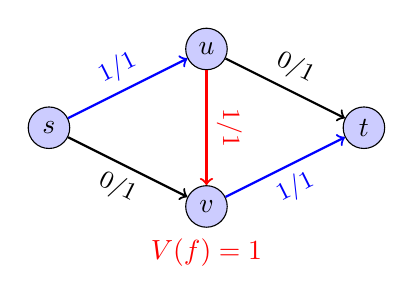
\begin{tikzpicture}[scale=1, auto,swap]

    \def\dx{0};
    \def\dy{0};	

     \foreach \x/\y/\name in { 0/0/s, 2/1/u, 2/-1/v, 4/0/t}
        \node[middlevertex, draw,  fill=blue!20] (\name) at (\x+\dx, \y+\dy) {$\name$};


    \foreach \source/ \dest /\weight in {s/u/{1/1}}
        \path[edge, sloped, midway, above, allow upside down, blue] (\source) -- node[weight] {\small $\weight$} (\dest);

    \foreach \source/ \dest /\weight in {u/t/{0/1}}
        \path[edge, sloped, midway, above, allow upside down] (\source) -- node[weight] {\small $\weight$} (\dest);

    \foreach \source/ \dest /\weight in {u/v/{1/1}}
        \path[edge, sloped, midway, above, allow upside down, red] (\source) -- node[weight] {\small $\weight$} (\dest);

    \foreach \source/ \dest /\weight in {v/t/{1/1}}
        \path[edge, sloped, midway, below, allow upside down, blue] (\source) -- node[weight] {\small $\weight$} (\dest);

    \foreach \source/ \dest /\weight in {s/v/{0/1}}
        \path[edge, sloped, midway, below, allow upside down] (\source) -- node[weight] {\small $\weight$} (\dest);
       \node[ultra thick, red, below] at (v.south) {$V(f)=1$};


%    \def\dx{5};
%    \def\dy{0};	
%
%     \foreach \x/\y/\name in { 0/0/s, 2/1/u, 2/-1/v, 4/0/t}
%        \node[middlevertex, draw,  fill=blue!20] (\name) at (\x+\dx, \y+\dy) {$\name$};
%
%
%    \foreach \source/ \dest /\weight in {s/u/{1/1}}
%        \path[edge, sloped, midway, above, allow upside down, blue] (\source) -- node[weight] {\small $\weight$} (\dest);
%
%    \foreach \source/ \dest /\weight in {u/t/{1/1}}
%        \path[edge, sloped, midway, above, allow upside down, blue] (\source) -- node[weight] {\small $\weight$} (\dest);
%
%    \foreach \source/ \dest /\weight in {u/v/{0/1}}
%        \path[edge, sloped, midway, above, allow upside down ] (\source) -- node[weight] {\small $\weight$} (\dest);
%
%    \foreach \source/ \dest /\weight in {v/t/{1/1}}
%        \path[edge, sloped, midway, below, allow upside down, blue] (\source) -- node[weight] {\small $\weight$} (\dest);
%
%    \foreach \source/ \dest /\weight in {s/v/{1/1}}
%        \path[edge, sloped, midway, below, allow upside down, blue] (\source) -- node[weight] {\small $\weight$} (\dest);
%
%    \node[ultra thick, red, below] at (v.south) {$V(f)=2$};

   \end{tikzpicture}
\end{figure}

 \item
  为了改进流$f$,我们应该使用一些手段 \textcolor{red}{\bf 更正在写错误}, 即 ``复原undo''边上做过的运输任务。
 \item 如何实现 "undo" 功能呢?
 \item   \textcolor{red}{\bf 增加反向边! }
 \item 假定我们增加一条 \textcolor{red}{\bf 反向} 边 $v\rightarrow u$ 到原始图. 接着我们可以更正这次运输,通过退回从$v$ 到 $u$的商品.
\end{itemize}


加了退货边的图就叫剩余图(Residual graph)。
\begin{figure}[H]
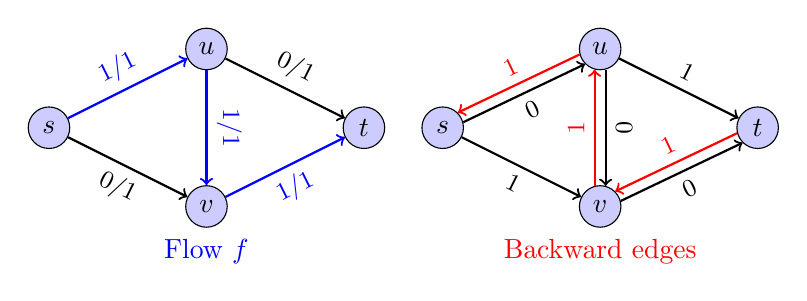
\begin{tikzpicture}[scale=1, auto,swap]

    \def\dx{0};
    \def\dy{0};	

     \foreach \x/\y/\name in { 0/0/s, 2/1/u, 2/-1/v, 4/0/t}
        \node[middlevertex, draw,  fill=blue!20] (\name) at (\x+\dx, \y+\dy) {$\name$};


    \foreach \source/ \dest /\weight in {s/u/{1/1}}
        \path[edge, sloped, midway, above, allow upside down, blue] (\source) -- node[weight] {\small $\weight$} (\dest);

    \foreach \source/ \dest /\weight in {u/t/{0/1}}
        \path[edge, sloped, midway, above, allow upside down] (\source) -- node[weight] {\small $\weight$} (\dest);

    \foreach \source/ \dest /\weight in {u/v/{1/1}}
        \path[edge, sloped, midway, above, allow upside down, blue] (\source) -- node[weight] {\small $\weight$} (\dest);

    \foreach \source/ \dest /\weight in {v/t/{1/1}}
        \path[edge, sloped, midway, below, allow upside down, blue] (\source) -- node[weight] {\small $\weight$} (\dest);

    \foreach \source/ \dest /\weight in {s/v/{0/1}}
        \path[edge, sloped, midway, below, allow upside down] (\source) -- node[weight] {\small $\weight$} (\dest);
       \node[ultra thick, blue, below] at (v.south) {Flow $f$};


    \def\dx{5};
    \def\dy{0};	

     \foreach \x/\y/\name in { 0/0/s, 2/1/u, 2/-1/v, 4/0/t}
        \node[middlevertex, draw,  fill=blue!20] (\name) at (\x+\dx, \y+\dy) {$\name$};

        \draw[->, thick] (s.15) -- node[below, sloped, midway] {\small $0$} (u.225);
        \draw[->, thick, red] (u.195) -- node[above, sloped, midway] {\small $1$} (s.45);

        \draw[->, thick] (u.285) -- node[above, sloped, midway] {\small $0$} (v.75);
        \draw[->, thick, red] (v.105) -- node[above, sloped, midway] {\small $1$} (u.255);

        \draw[->, thick] (v.15) -- node[below, sloped, midway] {\small $0$} (t.225);
        \draw[->, thick, red] (t.195) -- node[above, sloped, midway] {\small $1$} (v.45);


%    \foreach \source/ \dest /\weight in {s/u/{1/1}}
%        \path[edge, sloped, midway, above, allow upside down, blue] (\source) -- node[weight] {\small $\weight$} (\dest);

    \foreach \source/ \dest /\weight in {u/t/{1}}
        \path[edge, sloped, midway, above, allow upside down, black] (\source) -- node[weight] {\small $\weight$} (\dest);

%    \foreach \source/ \dest /\weight in {u/v/{0/1}}
%        \path[edge, sloped, midway, above, allow upside down ] (\source) -- node[weight] {\small $\weight$} (\dest);

%    \foreach \source/ \dest /\weight in {v/t/{1/1}}
%        \path[edge, sloped, midway, below, allow upside down, blue] (\source) -- node[weight] {\small $\weight$} (\dest);

    \foreach \source/ \dest /\weight in {s/v/{1}}
        \path[edge, sloped, midway, below, allow upside down, black] (\source) -- node[weight] {\small $\weight$} (\dest);

   \node[ultra thick, red, below] at (v.south) {Backward edges};

   \end{tikzpicture}
\end{figure}

\textbf{剩余图 Residual Graph}


   给定一个有向图$G=<V,E>$, 有一个流 $f$, 我们定义 \textcolor{red}{\bf 剩余图residual graph} $G_f=<V, E'>$. 对于任何一条边$e = (u,v) \in E$, 按照下面的要求将两条边加入到$E'$ :
\begin{enumerate}
\begin{small}
 \item (\textcolor{red}{\bf 正向边} $(u, v)$ 标注剩余的运输容量): \\
如果 $f(e) < C(e)$, 添加一条边$e=(u,v)$ 标注运输容量$C(e)=C(e) - f(e)$.
 \item (\textcolor{red}{\bf 反向边}  $(v, u)$ 标注回退容量): \\
如果 $f(e) > 0$, 添加一条边 $e'=(v,u)$ 标注回退容量 $C(e') = f(e)$.
\end{small}
\end{enumerate}

 \begin{figure}[H]
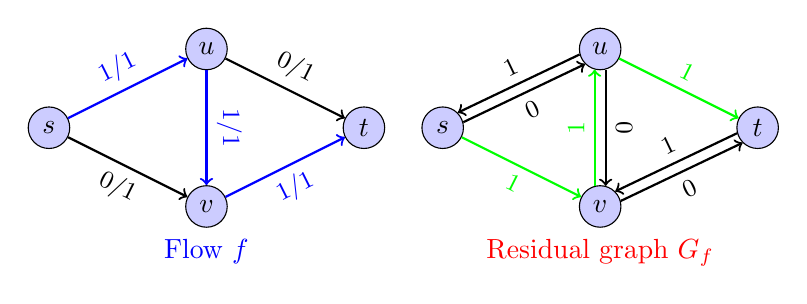
\begin{tikzpicture}[scale=1, auto,swap]

    \def\dx{0};
    \def\dy{0};	

     \foreach \x/\y/\name in { 0/0/s, 2/1/u, 2/-1/v, 4/0/t}
        \node[middlevertex, draw,  fill=blue!20] (\name) at (\x+\dx, \y+\dy) {$\name$};


    \foreach \source/ \dest /\weight in {s/u/{1/1}}
        \path[edge, sloped, midway, above, allow upside down, blue] (\source) -- node[weight] {\small $\weight$} (\dest);

    \foreach \source/ \dest /\weight in {u/t/{0/1}}
        \path[edge, sloped, midway, above, allow upside down] (\source) -- node[weight] {\small $\weight$} (\dest);

    \foreach \source/ \dest /\weight in {u/v/{1/1}}
        \path[edge, sloped, midway, above, allow upside down, blue] (\source) -- node[weight] {\small $\weight$} (\dest);

    \foreach \source/ \dest /\weight in {v/t/{1/1}}
        \path[edge, sloped, midway, below, allow upside down, blue] (\source) -- node[weight] {\small $\weight$} (\dest);

    \foreach \source/ \dest /\weight in {s/v/{0/1}}
        \path[edge, sloped, midway, below, allow upside down] (\source) -- node[weight] {\small $\weight$} (\dest);
       \node[ultra thick, blue, below] at (v.south) {Flow $f$};


    \def\dx{5};
    \def\dy{0};	

     \foreach \x/\y/\name in { 0/0/s, 2/1/u, 2/-1/v, 4/0/t}
        \node[middlevertex, draw,  fill=blue!20] (\name) at (\x+\dx, \y+\dy) {$\name$};

        \draw[->, thick] (s.15) -- node[below, sloped, midway] {\small $0$} (u.225);
        \draw[->, thick] (u.195) -- node[above, sloped, midway] {\small $1$} (s.45);

        \draw[->, thick] (u.285) -- node[above, sloped, midway] {\small $0$} (v.75);
        \draw[->, thick, green] (v.105) -- node[above, sloped, midway, green] {\small $1$} (u.255);

        \draw[->, thick] (v.15) -- node[below, sloped, midway] {\small $0$} (t.225);
        \draw[->, thick] (t.195) -- node[above, sloped, midway] {\small $1$} (v.45);


%    \foreach \source/ \dest /\weight in {s/u/{1/1}}
%        \path[edge, sloped, midway, above, allow upside down, blue] (\source) -- node[weight] {\small $\weight$} (\dest);

    \foreach \source/ \dest /\weight in {u/t/{1}}
        \path[edge, sloped, midway, above, allow upside down, green] (\source) -- node[weight] {\small $\weight$} (\dest);

%    \foreach \source/ \dest /\weight in {u/v/{0/1}}
%        \path[edge, sloped, midway, above, allow upside down ] (\source) -- node[weight] {\small $\weight$} (\dest);

%    \foreach \source/ \dest /\weight in {v/t/{1/1}}
%        \path[edge, sloped, midway, below, allow upside down, blue] (\source) -- node[weight] {\small $\weight$} (\dest);

    \foreach \source/ \dest /\weight in {s/v/{1}}
        \path[edge, sloped, midway, below, allow upside down, green] (\source) -- node[weight] {\small $\weight$} (\dest);

   \node[ultra thick, red, below] at (v.south) {Residual graph $G_f$};

   \end{tikzpicture}
\end{figure}
提示: 路径path中包含反向边 $(v,u)$。



\textbf{沿着路径增广流:从$f$ 到$f'$}
\begin{figure}[H]
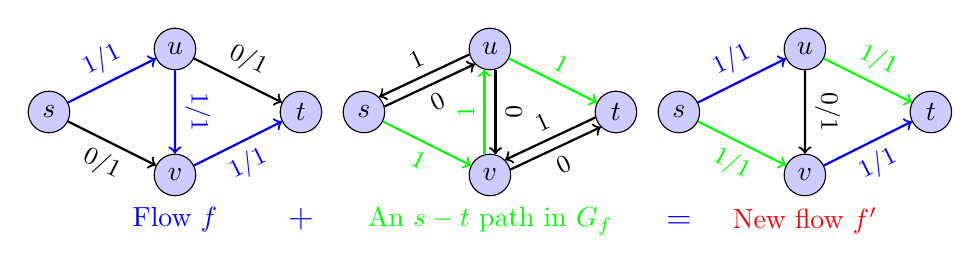
\begin{tikzpicture}[scale=0.8, auto,swap]

    \def\dx{0};
    \def\dy{0};	

     \foreach \x/\y/\name in { 0/0/s, 2/1/u, 2/-1/v, 4/0/t}
        \node[middlevertex, draw,  fill=blue!20] (\name) at (\x+\dx, \y+\dy) {$\name$};


    \foreach \source/ \dest /\weight in {s/u/{1/1}}
        \path[edge, sloped, midway, above, allow upside down, blue] (\source) -- node[weight] {\small $\weight$} (\dest);

    \foreach \source/ \dest /\weight in {u/t/{0/1}}
        \path[edge, sloped, midway, above, allow upside down] (\source) -- node[weight] {\small $\weight$} (\dest);

    \foreach \source/ \dest /\weight in {u/v/{1/1}}
        \path[edge, sloped, midway, above, allow upside down, blue] (\source) -- node[weight] {\small $\weight$} (\dest);

    \foreach \source/ \dest /\weight in {v/t/{1/1}}
        \path[edge, sloped, midway, below, allow upside down, blue] (\source) -- node[weight] {\small $\weight$} (\dest);

    \foreach \source/ \dest /\weight in {s/v/{0/1}}
        \path[edge, sloped, midway, below, allow upside down] (\source) -- node[weight] {\small $\weight$} (\dest);
       \node[ultra thick, blue, below] at (v.south) {Flow $f$};

       \node[ultra thick, blue] at (4, -1.7 ) {\large +};

    \def\dx{5};
    \def\dy{0};	

     \foreach \x/\y/\name in { 0/0/s, 2/1/u, 2/-1/v, 4/0/t}
        \node[middlevertex, draw,  fill=blue!20] (\name) at (\x+\dx, \y+\dy) {$\name$};

        \draw[->, thick] (s.15) -- node[below, sloped, midway] {\small $0$} (u.225);
        \draw[->, thick] (u.195) -- node[above, sloped, midway] {\small $1$} (s.45);

        \draw[->, thick] (u.285) -- node[above, sloped, midway] {\small $0$} (v.75);
        \draw[->, thick, green] (v.105) -- node[above, sloped, midway, green] {\small $1$} (u.255);

        \draw[->, thick] (v.15) -- node[below, sloped, midway] {\small $0$} (t.225);
        \draw[->, thick] (t.195) -- node[above, sloped, midway] {\small $1$} (v.45);


%    \foreach \source/ \dest /\weight in {s/u/{1/1}}
%        \path[edge, sloped, midway, above, allow upside down, blue] (\source) -- node[weight] {\small $\weight$} (\dest);

    \foreach \source/ \dest /\weight in {u/t/{1}}
        \path[edge, sloped, midway, above, allow upside down, green] (\source) -- node[weight] {\small $\weight$} (\dest);

%    \foreach \source/ \dest /\weight in {u/v/{0/1}}
%        \path[edge, sloped, midway, above, allow upside down ] (\source) -- node[weight] {\small $\weight$} (\dest);

%    \foreach \source/ \dest /\weight in {v/t/{1/1}}
%        \path[edge, sloped, midway, below, allow upside down, blue] (\source) -- node[weight] {\small $\weight$} (\dest);

    \foreach \source/ \dest /\weight in {s/v/{1}}
        \path[edge, sloped, midway, below, allow upside down, green] (\source) -- node[weight] {\small $\weight$} (\dest);

   \node[ultra thick, green, below] at (v.south) {An $s-t$ path in $G_f$};


      \node[ultra thick, blue] at (10, -1.75) {\large =};


    \def\dx{10};
    \def\dy{0};	

     \foreach \x/\y/\name in { 0/0/s, 2/1/u, 2/-1/v, 4/0/t}
        \node[middlevertex, draw,  fill=blue!20] (\name) at (\x+\dx, \y+\dy) {$\name$};

%        \draw[->, thick] (s.15) -- node[below, sloped, midway] {\small $0$} (u.225);
%        \draw[->, thick] (u.195) -- node[above, sloped, midway] {\small $1$} (s.45);
%
%        \draw[->, thick] (u.285) -- node[above, sloped, midway] {\small $0$} (v.75);
%        \draw[->, thick, green] (v.105) -- node[above, sloped, midway, green] {\small $1$} (u.255);
%
%        \draw[->, thick] (v.15) -- node[below, sloped, midway] {\small $0$} (t.225);
%        \draw[->, thick] (t.195) -- node[above, sloped, midway] {\small $1$} (v.45);


    \foreach \source/ \dest /\weight in {s/u/{1/1}}
        \path[edge, sloped, midway, above, allow upside down, blue] (\source) -- node[weight] {\small $\weight$} (\dest);

    \foreach \source/ \dest /\weight in {u/t/{1/1}}
        \path[edge, sloped, midway, above, allow upside down, green] (\source) -- node[weight] {\small $\weight$} (\dest);

    \foreach \source/ \dest /\weight in {u/v/{0/1}}
        \path[edge, sloped, midway, above, allow upside down ] (\source) -- node[weight] {\small $\weight$} (\dest);

    \foreach \source/ \dest /\weight in {v/t/{1/1}}
        \path[edge, sloped, midway, below, allow upside down, blue] (\source) -- node[weight] {\small $\weight$} (\dest);

    \foreach \source/ \dest /\weight in {s/v/{1/1}}
        \path[edge, sloped, midway, below, allow upside down, green] (\source) -- node[weight] {\small $\weight$} (\dest);

   \node[ultra thick, red, below] at (v.south) {New flow $f'$};



   \end{tikzpicture}
\end{figure}

注释:

\begin{itemize}
\item
通过使用反向边 $v\rightarrow u$, 原始的从 $u$ 到 $v$的运输被退回.
\item 更具体的,
 第一次商品运输流$f$将会改变它的路径(从$s\rightarrow u\rightarrow v\rightarrow t$ 到 $s\rightarrow u\rightarrow t$),当第二次使用路 $s\rightarrow v\rightarrow t$的时候.
 \end{itemize}


\end{CJK}
\end{document}


